%
% chapter.tex -- Beschreibung des Inhaltes
%
% (c) 2021 Prof Dr Andreas Müller, Hochschule Rapperswil
%
% !TeX spellcheck = de_CH
\chapter{Spezielle Funktionen und Rekursion
\label{buch:chapter:rekursion}}
\kopflinks{Spezielle Funktionen und Rekursion}
Die Fakultät $n!=1\cdot 2\cdots n$ ist eine ersten Funktionen, für die
man normalerweise auch eine rekursive Definition kennenlernt.
Rekursion ist eine besonders gut der numerischen Berechnung zugängliche
Art, spezielle Funktionen zu definieren.
In diesem Kapitel sollen daher in
Abschnitt~\ref{buch:rekursion:section:gamma}
zunächst die Gamma-Funktion als Verallgemeinerung konstruiert
und charakterisiert werden.
Die Beta-Funktion in
Abschnitt~\ref{buch:rekursion:gamma:section:beta}
verallgemeinert diese Rekursionsbeziehungen.
Abschnitt~\ref{buch:rekursion:section:linear}
erinnert an die Methoden, mit denen lineare Rekursionsgleichungen
gelöst werden können. 
Erfüllten die Koeffizienten einer Potenzreihe eine spezielle
Rekursionsbeziehung, entsteht die besonders vielfältige Familie
der hypergeometrischen Funktionen, die in
Abschnitt~\ref{buch:rekursion:section:hypergeometrische-funktion}
eingeführt werden.

%
% 1-gamma.tex -- Abschnitt über die Gamma-funktion
%
% (c) 2021 Prof Dr Andreas Müller, OST Ostschweizer Fachhochschule
%
\section{Die Gamma-Funktion
\label{buch:rekursion:section:gamma}}
\kopfrechts{Die Gamma-Funktion}
Die Fakultät $x!$ kann rekursiv durch 
\[
	x! = x\cdot (x-1)! \qquad\text{und}\qquad 0!=1
\]
für alle natürlichen Zahlen $x\in\mathbb{N}$ definiert werden.
Äquivalent damit ist eine Funktion 
\begin{equation}
\Gamma(x+1) = x\Gamma(x)
\qquad\text{und}\qquad 
\Gamma(1)=1.
\label{buch:rekursion:eqn:gammadef}
\end{equation}
Kann man eine reelle oder komplexe Funktion finden, die die
Funktionalgleichung~\eqref{buch:rekursion:eqn:gammadef}
\index{Gamma-Funktion!Funktionalgleichung}%
\index{Funktionalgleichung der Gamma-Funktion}%
erfüllt und damit die Fakultät auf beliebige Argumente ausdehnt?

%
% Definition als Grenzwert
%
\subsection{Definition als Grenzwert}
Die Fakultät $n!$ ist ein Produkt von $n$ Faktoren, es ist daher
natürlich zu versuchen, auch $x!$ als ein Produkt zu schreiben.
Allerdings kann es nicht möglich sein, dies mit einer endlichen
Anzahl von Faktoren zu machen, denn wenn $x$ grösser wird, muss auch
die Zahl der Faktoren grösser werden.
Mit jedem zusätzlichen Faktor ist ein Sprung der Werte zu erwarten.
Wir erwarten daher entweder ein unendliches Produkt oder einen
Ausdreck, bei dem die ``Anzahl'' $x$ der Faktoren im Exponenten
steht.
In diesem Abschnitt soll zunächst eine solcher Ausdruck gefunden
werden.
Dieser ist jedoch für die numerische Berechnung absolut ungeeignet,
so dass er später in ein unendliches Produkt umgeformt werden muss.

%
% Fakultät als Bruch
%
\subsubsection{Fakultät als Bruch}
Euler hat das Problem, die Fakultät auf beliebige reelle oder komplexe
Zahlen auszudehnen, wie folgt angepackt.
Zunächst hat er bemerkt, dass für ganzzahlige $x$ und natürliche $n$
\begin{align}
x! 
&=
1\cdot 2\cdot 3\cdot\ldots\cdot x
\notag
\\
&=
\frac{
1\cdot 2\cdot 3\cdot\ldots\cdot x\cdot (x+1) (x+2)\cdots(x+n)
}{
(x+1)(x+2)\cdots(x+n)
}
\notag
\\
&=
\frac{
1\cdot 2\cdot\ldots\cdot n\cdot(n+1)\cdot(n+2)\cdots(n+x)
}{
(x+1)(x+2)\cdots(x+n)
}
\notag
\\
&=
\frac{n! \cdot (n+1)(n+1)\cdots(n+x)}{(x+1)(x+2)\cdots(x+n)}
\label{buch:rekursion:gamma:eqn:fakultaet}
\end{align}
gilt.
Der Plan ist, dies so umzuformen, dass man für $x$ eine beliebige
komplexe Zahl einsetzen kann.

%
% Pochhammer-Symbol
%
\subsubsection{Pochhammer-Symbol}
Die spezielle Form des Nenners und des zweiten Faktors im Zähler
von \eqref{buch:rekursion:gamma:eqn:fakultaet}
rechtfertigt die folgende Definition.

\begin{definition}[Pochhammer]
Für $a\in\mathbb{C}$ und $n\in\mathbb{N}$ heisst das Produkt
\[
(a)_n = a\cdot(a+1)\cdot(a+2)\cdots(a+n-1)
\]
das Pochhammer-Symbol oder die verschobene Fakultät.
\index{Pochhammer-Symbol}
\end{definition}

Die verschobene Fakultät $(a)_n$ hat also genau $n$ Faktoren, deren
erster $1$ ist.
Die gewöhnliche Fakultät hat $n$ Faktoren, deren erster $1$ ist, also
ist $n! = (1)_n$.

Der Ausdruck \eqref{buch:rekursion:gamma:eqn:fakultaet}
für $x!$ wird unter Verwendung des Pochhammer-Symbols zu
\begin{equation}
x! = \frac{n! (n+1)_x}{(x+1)_n}.
\label{buch:rekursion:gamma:eqn:produkt2}
\end{equation}
Leider ist dieser Ausdruck ebenfalls nicht auf beliebige $x$
verallgemeinerungsfähig, denn $(n)_x$ ist nur natürliche $x$ definiert.
Der Faktor $(n+1)_x$ enthält $x$ Faktoren beginnend bei $n$.
Für grosses $n$ sind diese Faktoren nahe beeinander, man sollte also
$(n+1)_x$ durch $n^x$ approximieren können.
Wir erweitern daher \eqref{buch:rekursion:gamma:eqn:produkt2} mit $n^x$
und erhalten
\begin{equation}
x!
=
\frac{n!\,n^x}{(x+1)_n}\cdot
\frac{(n+1)_x}{n^x}.
\label{buch:rekursion:gamma:eqn:produkt3}
\end{equation}
Der erste Faktor in diesem Ausdruck enthält jetzt nur noch Dinge,
die für beliebige $x\in\mathbb{C}$ definiert sind.

%
% Grenwertdefinition
%
\subsubsection{Grenzwertdefinition}
Der zweite Bruch in \eqref{buch:rekursion:gamma:eqn:produkt3}
besteht aus Termen, die zwar nur für natürliches $x$ definiert sind,
wir vermuten aber, dass er für grosses $n$ gegen $1$ konvergiert.
Tatsächlich gilt
\[
\lim_{n\to\infty}
\frac{(n+1)_x}{n^x}
=
\lim_{n\to\infty}
\underbrace{\frac{n+1}{n}}_{\displaystyle\to 1}
\cdot
\underbrace{\frac{n+2}{n}}_{\displaystyle\to 1}
\cdot\ldots\cdot
\underbrace{\frac{n+x}{n}}_{\displaystyle\to 1}
=
1,
\]
da  $(n+x)/n=1+x/n\to 1$ für grosses $n$.
Dies würde die folgende Definition rechtfertigen.

\begin{definition}
\label{buch:rekursion:gamma:def:definition}
Die Gamma-Funktion $\Gamma(x)$ einer Zahl
$x\in\mathbb{C}\setminus\{0,-1,-2,-3,\dots\}$ ist der Grenzwert
\[
\Gamma(x) = \lim_{n\to\infty} \frac{n!\,n^{x-1}}{(x)_n}.
\] 
\index{Grenzwertdefinition der Gamma-Funktion}%
\index{Gamma-Funktion!Grenzwertdefinition}%
\end{definition}

%
% Rekursionsgleichung für Gamma(x)
%
\subsubsection{Rekursionsgleichung für $\Gamma(x)$}
Es ist aus der Herleitung klar, dass $\Gamma(n)=(n-1)!$ sein muss.
Wir sollten dies aber auch direkt aus der
Definition~\ref{buch:rekursion:gamma:def:definition} ableiten
können.
Dazu müssen wir nur überprüfen, ob $\Gamma(1)=0!=1$ ist und ob
die Rekursionsformel $\Gamma(n)=n\Gamma(n-1)$ gilt.

Den Wert $\Gamma(1)$ kann man direkt berechnen:
\[
\Gamma(1)
=
\lim_{n\to\infty} \frac{n!}{(1)_n}
=
\lim_{n\to\infty} \frac{n!}{n!}
=
1
\]
wegen $(1)_n=n!$.

Für die Rekursionsformel muss man den Grenzwert für $x$ und $x+1$
miteinander vergleichen.
Aus dem Term $(x+1)_n$ im Nenner muss man einen Term $(x)_n$ machen,
dies ist möglich, indem man mit $x$ erweitert:
\begin{align*}
\Gamma(x+1)
&=
\lim_{n\to\infty}\frac{n!\,n^x}{(x+1)_n}
=
x\lim_{n\to\infty}\frac{n!\,n^x}{x(x+1)_n}
=
x\lim_{n\to\infty}\frac{n!\,n^x}{(x)_{n+1}}.
\intertext{Wir müssen jetzt nur noch zeigen, dass der Grenzwert
auf der rechten Seite gegen $\Gamma(x)$ konvergiert,
in dessen Definition aber die Potenz $n^{x-1}$ vorkommt.
Wir müssen also einen Faktor $n$ los werden und gleichzeitig
aus $n$ überall $n+1$ machen, damit der Nenner wieder passt.
Dabei wird}
\Gamma(x+1)
&=
x\lim_{n\to\infty}
\frac{(n+1)!n^{x-1}}{(x)_{n+1}}
\cdot
\underbrace{\frac{n}{n+1}}_{\displaystyle\to 1}
\\
&=
x\lim_{n\to\infty}
\underbrace{\frac{(n+1)!(n+1)^{x-1}}{(x)_{n+1}}}_{\displaystyle\to\Gamma(x)}
\cdot
\frac{n^{x-1}}{(n+1)^{x-1}}
\\
&=
x
\Gamma(x)
\lim_{n\to\infty} \biggl(\frac{n}{n+1}\biggr)^{x-1}
=
x\Gamma(x),
\end{align*}
Weil $n/(n+1)\to 1$ ist und die Funktion $z\mapsto z^{x-1}$ für alle
nach der Definition zulässigen Werte von $x$ eine stetige Funktion ist.

%
% Gamma-Funktion und Pochhammer-Symbol
%
\subsubsection{Gamma-Funktion und Pochhammer-Symbol}
Durch Iteration der Rekursionsformel für $\Gamma(x)$ folgt jetzt
\begin{align*}
\Gamma(x+n)
&=
(x+n-1) \Gamma(x+n-1)
\\
&=
(x+n-1)(x+n-2)\Gamma(x+n-2)
\\
&=
\underbrace{
(x+n-1)(x+n-2)\cdots(x-1)(x)
}_{\text{$n$ Faktoren}} \Gamma(x)
\\
&=(x)_n \Gamma(x).
\end{align*}
Damit folgt

\begin{satz}
\index{Satz!Pochhammer-Symbol@Pochhammer-Symbol und $\Gamma(x)$}%
\label{buch:rekursion:gamma:satz:gamma-pochhammer}
Die Rekursionsformel für die Gamma-Funktion kann geschrieben werden als
\[
\Gamma(x+n) = (x)_n \Gamma(x).
\]
Das Pochhammer-Symbol $(x)_n$ ist für alle natürlichen $n$ gegeben durch
\[
(x)_n = \frac{\Gamma(x+n)}{\Gamma(x)}.
\]
\end{satz}

%
% Numerische Unzulänglichkeit der Grenzwertdefinition
%
\subsubsection{Numerische Unzulänglichkeiten der Grenzwertdefinition}
\begin{table}
\centering
%\renewcommand{\arraystretch}{1.1}
\begin{tabular}{|>{$}c<{$}|>{$}r<{$}|>{$}l<{$}|>{$}l<{$}|}
\hline
\log_{10} n&           n&n!n^{x-1}/(x)_n\mathstrut     &       \text{Fehler%
\vrule height12pt depth6pt width0pt} \\
\hline
\text{\vrule height12pt depth0pt width0pt} 
          1&          10&1.\underline{7}947392559855804&0.0222854050800643\\
          2&         100&1.\underline{77}46707942830697&0.0022169433775536\\
          3&        1000&1.\underline{772}6754214755178&0.0002215705700017\\
          4&       10000&1.\underline{7724}760067171375&0.0000221558116213\\
          5&      100000&1.\underline{77245}60664742375&0.0000022155687214\\
          6&     1000000&1.\underline{77245}40724623101&0.0000002215567940\\
          7&    10000000&1.\underline{7724538}730613721&0.0000000221558560\\
          8&   100000000&1.\underline{77245385}31233258&0.0000000022178097\\
          9&  1000000000&1.\underline{77245385}11320680&0.0000000002265519\\
         10& 10000000000&1.\underline{772453850}9261316&0.0000000000206155\\
         11&100000000000&1.\underline{77245385}14549788&0.0000000005494627\\
           &      \infty&1.\underline{7724538509055161}&
\text{\vrule height12pt depth6pt width0pt} \\
\hline
\end{tabular}
\caption{Numerische Berechnung mit der Grenzwertdefinition
und rekursiver Berechnung von $n!/(x)_n$ mit Hilfe der Folge
\eqref{buch:rekursion:gamma:pnfolge}.
Die Konvergenz ist sehr langsam, die Anzahl korrekter Stellen
wächst logarithmisch mit $n$.
\label{buch:rekursion:gamma:produktberechnung}}
\end{table}
Die Grenzwertdefinition~\ref{buch:rekursion:gamma:def:definition}
ist zwar zweifellos richtig, kann aber nicht für die numerische 
Berechnung der Gamma-Funktion verwendet werden.
Die Existenz des Grenzwertes verwendet, dass $x\ll n$ sein muss,
damit $(n+x)/n$ gegenüber $1$ vernachlässigt werden kann.
Die Grenzwertdefinition beginnt also erst, vernünftige Approximationen
von $\Gamma(x)$ zu geben, wenn $n$ viel grösser also $x$ ist.
Andererseits wächst $n!$ sehr schnell an, schon für $n=171$ ist
das Resultat grösser als was der \texttt{double}-Datentyp fassen kann.
Dies ist aber viel zu kleine, um gute Approximationen auch für kleine
Werte von $x$ zu geben.
So findet man zum Beispiel für $x=\frac12$ und $n=170$ mit Octave
\[
\frac{n!\,n^{x-1}}{(x)_n}
=
\frac{170!}{\sqrt{170}\cdot \frac12\cdot\frac32\cdot\ldots\cdot\frac{339}{2}}
=
\frac{7.2574\cdot10^{307}}{13.308\cdot 3.1381\cdot10^{305}}
=
1.7738.
\]
Andererseits werden wir später sehen, dass 
\[
\Gamma({\textstyle\frac12})
=
\sqrt{\pi}
=
1.772453850905516
\]
ist.
Die Approximation mit Hilfe der Grenzwertdefinition kann also
grundsätzlich nicht mehr als zwei korrekte Nachkommastellen liefern.

Den Quotienten $n!/(x)_n$ kann man mit Hilfe der Rekursionsformel
\begin{equation}
p_n = p_{n-1}\cdot \frac{n}{x+n-1},\qquad
p_0 = 0
\label{buch:rekursion:gamma:pnfolge}
\end{equation}
etwas effizienter berechnen. 
Insbesondere umgeht man damit das Problem, dass $n!$ den Wertebereich 
des \texttt{double} Datentyps sprengt.
Der Wert der Gamma-Funktion kann dann durch $p_nn^{x-1}$ approximiert
werden.
Die Tabelle~\ref{buch:rekursion:gamma:produktberechnung} fasst die
Resultate zusammen und zeigt, dass die Konvergenz logarithmisch ist:
die Anzahl korrekter Nachkommastellen ist $\log_{10}n$.

%
% Produktformel
%
\subsection{Produktformel}
Ein möglicher Ausweg aus den numerischen Schwierigkeiten mit der
Grenzwertdefinition ist, den schnell wachsenden Faktor $n!$
in den Zähler zu bringen, so dass er der Konvergenz etwas nachhilft.
Wir berechnen daher den Kehrwert $1/\Gamma(x)$.

\begin{satz}
\index{Satz!Produktformel@Produktformel für $\Gamma(x)$}%
\label{buch:rekursion:gamma:satz:produktformel}
Der Kehrwert der Gamma-Funktion kann geschrieben werden als
\begin{equation}
\frac{1}{\Gamma(x)}
=
xe^{\gamma x}
\prod_{k=1}^\infty
\biggl(1+\frac{x}k\biggr)\,e^{-\frac{x}{k}},
\label{buch:rekursion:gamma:eqn:produktformel}
\index{Gamma-Funktion!Produktformel}%
\end{equation}
wobei $\gamma$ die Euler-Mascheronische Konstante
\index{Euler-Mascheronische Konstante}%
\[
\gamma
=
\lim_{n\to\infty}
\biggl(\sum_{k=1}^n\frac{1}{k}-\log n\biggr)
\]
ist.
\index{Gamma-Funktion!Produktformel}%
\index{Produktformel für die Gamma-Funkion}%
\end{satz}

\begin{proof}[Beweis]
Es sind zwei Dinge nachzuprüfen.
Zunächst muss nachgewiesen werden, dass das unendliche Produkt 
überhaupt konvergiert.
Wenn das gesichert ist, muss noch gezeigt werden, dass der Grenzwert
tatsächlich $1/\Gamma(x)$ ist.

Für die Konvergenz beachtet man, dass die Faktoren des Produkts 
die Form
\begin{align*}
\biggl(1+\frac{x}n\biggr)e^{-\frac{x}{n}}
&=
\biggl(1+\frac{x}n\biggr)
\biggl(1-\frac{x}{n}+\frac{x^2}{2n^2}-\frac{x^3}{3!n^3}+\dots\biggr)
\\
&=
1-\frac{x^2}{n^2} + 
\biggl(1+\frac{x}n\biggr)
\biggl(\frac{x^2}{2n^2}-\dots\biggr)
\\
&=
1-\frac{x^2}{n^2} + \frac{x^2}{2n^2} + O\bigl((\textstyle\frac{x}{n})^2\bigr)
\\
&=
1-\frac{x^2}{2n^2} + O\bigl((\textstyle\frac{x}{n})^3\bigr)
\end{align*}
haben.
Da die Reihe 
\[
\sum_{n=1}^\infty \frac{x^2}{n^2}
\]
konvergent ist, konvergiert auch das Produkt.
% XXX wir brauchen irgendwo das Konvergenzkriterium für ein Produkt

Um die Übereinstimmung der Produktformel mit $1/\Gamma(x)$ zu zeigen,
berechnen wir
\begin{align*}
\frac{1}{\Gamma(x)}
&=
\lim_{n\to\infty} 
\frac{(x)_n}{n!\,n^{x-1}}
=
\lim_{n\to\infty} 
\frac{x(x+1)(x+2)\cdots(x+n-1)}{1\cdot 2\cdot3\cdots (n-1)\cdot n\cdot n^{x-1}}
\\
&=
x
\lim_{n\to\infty} 
\frac{x+1}{1}
\cdot
\frac{x+2}{2}
\cdots
\frac{x+n-1}{n-1}
\cdot
n^{-x}
\\
&=
x
\lim_{n\to\infty}
\biggl(1+\frac{x}{1}\biggr)
\cdot
\biggl(1+\frac{x}{2}\biggr)
\cdots
\biggl(1+\frac{x}{n-1}\biggr)
\cdot
e^{-x\log n}
\\
&=
x
\prod_{k=1}^{n-1}
\biggl(1+\frac{x}{k}\biggr)
e^{-\frac{x}{k}}
e^{\frac{x}{k}}
e^{-x\log n}
\\
&=
x
\biggl(
\lim_{n\to\infty}
\prod_{k=1}^{n-1}
\biggl(1+\frac{x}{k}\biggr)
e^{-\frac{x}{k}}
\biggr)
\cdot
\biggl(
\lim_{n\to\infty}
e^{x\bigl(\sum_{k=1}^{n-1}\frac{1}{k} - \log n\bigr)}
\biggr)
\end{align*}
Der Klammerausdruck im Exponent des letzten Faktors auf der rechten Seite
konvergiert nach Definition der Euler-Mascheronischen Konstanten gegen
$\gamma$, somit folgt 
\[
\frac{1}{\Gamma(x)}
=
xe^{\gamma x}\prod_{k=1}^\infty \biggl(1+\frac{x}{k}\biggr)e^{-\frac{x}{k}},
\]
wie behauptet.
Damit ist Satz~\ref{buch:rekursion:gamma:satz:produktformel}
vollständig bewiesen.
\end{proof}

\begin{table}
\centering
\begin{tabular}{|>{$}c<{$}|>{$}r<{$}|>{$}c<{$}|>{$}c<{$}|}
\hline
k & n &  \Gamma(\frac12,n) & \Gamma(\frac12) - \Gamma(\frac12,n)%
\text{\vrule height12pt depth6pt width0pt} \\
\hline
\text{\vrule height12pt depth0pt width0pt} 
     1&     10& 1.\underline{7}518166478& -0.0206372031 \\
     2&    100& 1.\underline{77}02543372& -0.0021995137 \\
     3&   1000& 1.\underline{772}2324556& -0.0002213953 \\
     4&  10000& 1.\underline{7724}316968& -0.0000221541 \\
     5& 100000& 1.\underline{77245}16354& -0.0000022156 \\
     6&1000000& 1.\underline{772453}6293& -0.0000002216 \\
\infty&       & 1.\underline{7724538509}&
\text{\vrule height12pt depth6pt width0pt} \\
\hline
\end{tabular}
\caption{Werte $\Gamma(\frac12,n)$ von $\Gamma(\frac12)$ berechnet mit
$n=10^k$ Faktoren der
Produktformel~\eqref{buch:rekursion:gamma:eqn:produktformel}
und der zugehörige Fehler.
Die korrekten Nachkommastellen sind unterstrichen.
Die Konvergenz ist genau gleich langsam wie in der Berechnung mit
Hilfe der Grenzwert-Definition in
Tabelle~\ref{buch:rekursion:gamma:produktberechnung}.
\label{buch:rekursion:gamma:gammatabelle}}
\end{table}

Um zu zeigen, dass die Produktform tatsächlich besser geeignet ist,
sind in der Tabelle~\ref{buch:rekursion:gamma:gammatabelle}
die Resultate der numerischen Rechnung  bis $n=1000000$ zusammengestellt.
Die Produktformel kann gute Werte von $\Gamma(x)$ auch für derart grosse
Werte von $n$ problemlos berechnen.

Der Fehler der numersichen Approximation ist von der Grössenordnung
$O(1/n)$ wie das auf Grund des verwendeten Konvergenzkriteriums
zu erwarten war.
Die Anzahl zu berücksichtigender Terme wächst daher exponentiall
mit der Anzahl gewünschter Stellen an, was für praktische Zwecke
zu langsam ist.
Für die numersiche Berechnung der Gamma-Funktion ist die Produktformel
daher im Allgemeinen nicht geeignet.

%
% Integralformel für die Gamma-Funktion
%
\subsection{Integralformel für die Gamma-Funktion}
Euler hat die folgende Integraldefinition der Gamma-Funktion gegeben.

\begin{definition}
\label{buch:rekursion:def:gamma}
Die Gamma-Funktion ist die Funktion 
\begin{equation}
\Gamma
\colon
\{z\in\mathbb{C} \mid \operatorname{Re}z>0\}
\to \mathbb{C}
:
z
\mapsto
\Gamma(z) = \int_0^\infty t^{z-1}e^{-t}\,dt
\label{buch:rekursion:eqn:gammaintegral}
\end{equation}
\index{Gamma-Funktion!Integraldefinition}%
\index{Integraldefinition der Gamma-Funktion}%
\end{definition}

Man beachte, dass das Integral für $x=0$ nicht definiert ist, eine
Potenzreihenentwicklung um einen Punkt $x_0$ auf der positiven reellen
Achse kann also höchstens den Konvergenzradius $\varrho=|x_0|$ haben.

Die Definition~\ref{buch:rekursion:def:gamma} wird erst später in
\eqref{buch:rekursion:gamma:integralbeweis} auf
Seite~\pageref{buch:rekursion:gamma:integralbeweis} gegeben.
Im Folgenden wird zunächst verifiziert, dass die Integraldarstellung
die richtigen Werte für natürliche Argumente hat, es wird aber auch
gezeigt, dass dies nicht ausreicht um zu schliessen, dass die
Integralformel mit der früher definierten Gamma-Funktion übereinstimmt.

%
% Funktionalgleichung für die Integraldefinition
%
\subsubsection{Funktionalgleichung für die Integraldefinition}
Tatsächlich ist es einfach nachzuprüfen, dass die Funktionalgleichung
der Gamma-Funktion auch für die Definition~\ref{buch:rekursion:def:gamma}
Korrekt ist. 
Dazu ist zunächgst nachzurechnen, dass mindestens ein Wert der neuen 
Definition übereinstimmt mit der alten Definnition, zum Beispiel der
Wert
\[
\Gamma(1)
=
\int_0^\infty t^{1-1}e^{-t}\,dt
=
\biggl[ -e^{-t} \biggr]_0^\infty
=
1.
\]
Ausserdem muss die Funktionalgleichung erfüllt sein, also
\begin{align*}
\Gamma(z)
&=
\int_0^\infty
\underbrace{t^{z-1}}_{\displaystyle\uparrow}
\underbrace{e^{-t}}_{\displaystyle\downarrow}
\,dt
=
\underbrace{\biggl[
\frac{1}{z} t^z e^{-t}
\biggr]_0^\infty}_{\displaystyle=0}
+
\frac{1}{z}
\int_0^\infty
t^z e^{-t}
\,dt
=
\frac{1}{z}\Gamma(z+1)
\\
\Rightarrow\qquad
z\Gamma(z)&=\Gamma(z+1).
\end{align*}
Dies beweist aber nur, dass die beiden Definitionen für positiv
ganzzahlige Argumente übereinstimmen.
Der folgende Abschnitt macht deutlich, dass es sehr viele Funktionen gibt,
die ebenfalls die Funktionalgleichung erfüllen.
Eine vollständige Rechtfertigung für diese Definition wird später
in Abschnitt~\ref{buch:rekursion:gamma:subsection:integralbeweis}
in Formel~\eqref{buch:rekursion:gamma:integralbeweis}
auf Seite~\pageref{buch:rekursion:gamma:integralbeweis}
gegeben.

\begin{figure}
\centering
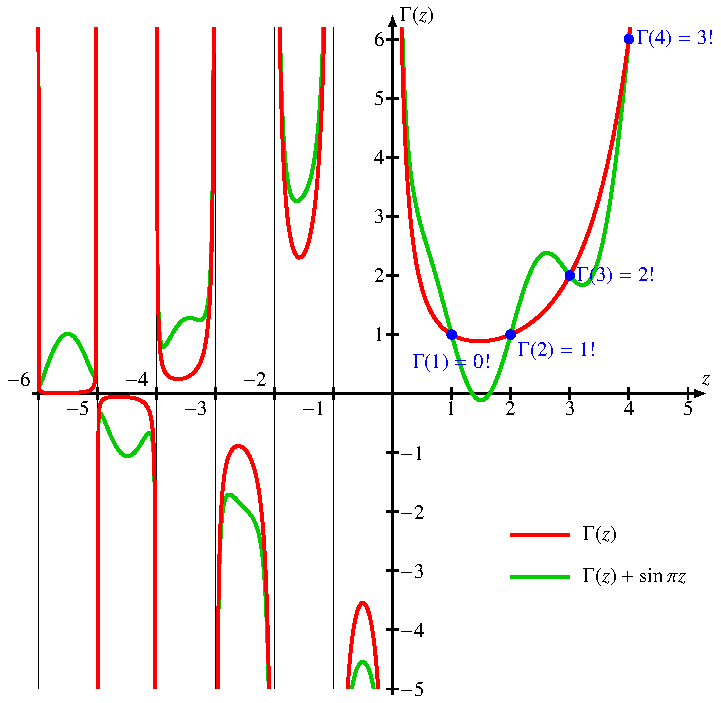
\includegraphics{chapters/040-rekursion/images/gammaplot.pdf}
\caption{Graph der Gamma-Funktion $z\mapsto\Gamma(z)$ und der alternativen
Funktion $\Gamma(z)+\sin(\pi z)$, die für ganzzahlige Argumente ebenfalls
die Werte der Fakultät annimmt.
\label{buch:rekursion:fig:gamma}}
\end{figure}

%
% Der Wert Gamma(1/2)
%
\subsubsection{Der Wert $\Gamma(\frac12)$}
Die Integraldarstellung kann dazu verwendet werden, $\Gamma(\frac12)$ 
zu berechnen.
\index{Gamma-Funktion!WertGamma12@Wert von $\Gamma(\frac12)$}%
\index{G(1/2)@$\Gamma(\frac12)$}%
Dazu verwendet man die Substition $t=s^2$ in der Integraldefinition
der Gamma-Funktion und berechnen
\begin{align}
\Gamma({\textstyle\frac12})
&=
\int_0^\infty t^{-\frac12} e^{-t}\,dt
=
\int_0^\infty s^{-1} e^{-s^2}\cdot 2s\,ds
=
2\int_0^\infty e^{-s^2}\,ds
=
\int_{-\infty}^\infty e^{-s^2}\,ds
=
\sqrt{\pi}.
\label{buch:rekursion:gamma:wert12}
\end{align}
Der Integrand im letzten Integral ist die Wahrscheinlichkeitsdichte
einer Normalverteilung, deren Integral wohlbekannt ist.

%
% Alternative Lösungen
%
\subsubsection{Alternative Lösungen der
Funktionalgleichung~\ref{buch:rekursion:eqn:gammadef}}
Die Funktion $\Gamma(z)$ ist nicht die einzige Funktion, die natürlichen
Zahlen die Werte $\Gamma(n+1) = n!$ der Fakultät annimmt.
Indem man eine beliebige Funktion $f(z)$ addiert, die auf alle
natürlichen Zahlen verschwindet, also $f(n)=0$ für $n\in\mathbb{N}$,
erhält man eine weitere Funktion, die auf natürlichen Zahlen
die Werte der Fakultät annimmt.
Ein Beispiel einer solchen Funktion ist
\begin{equation}
z\mapsto f(z)=\Gamma(z) + \sin \pi z,
\label{buch:rekursion:eqn:gammaalternative}
\end{equation}
die Funktion $f(z)=\sin\pi z$ verschwindet sogar auf allen ganzen
Zahlen.

In Abbildung~\ref{buch:rekursion:fig:gamma} ist die Gamma-Funktion
in rot geplotet, die Funktion~\eqref{buch:rekursion:eqn:gammaalternative}
in grün.
Die Punkte $(n,(n-1)!)$ sind in blau bezeichnet, sie sind beiden Graphen
gemeinsam.

In Abschnitt~\ref{buch:funktionentheorie:subsection:satz-von-carlson}
wir mit Mitteln der komplexen Funktionentheorie gezeigt, dass eine
Funktion, die für ganzzahlige Argument mit $\Gamma(x)$ zusammenfällt
und sich im Rest der rechten Halbebene nur durch eine beschränkte
Funktion von $\Gamma(x)$ unterscheidet, mit $\Gamma(x)$
identisch sein muss.
Von Wielandt stammt das folgende, noch etwas speziellere Resultat,
welches hier nicht bewiesen wird.

\begin{satz}[Wielandt]
\index{Satz!von Wielandt}%
\index{Wielandt, Satz von}%
Ist $f(z)$ eine für $\operatorname{Re}z>0$ definiert Funktion mit
den folgenden drei Eigenschaften
\begin{enumerate}
\item $f(1)=1$
\item $f(z+1)=zf(z)$ für $\operatorname{Re}z>0$
\item $f(z)$ ist beschränkt im Streifen $1\le \operatorname{Re}z< 2$
\end{enumerate}
Dann ist $ f(z) = \Gamma(z) $.
\end{satz}

% XXX Gamma in the interval (1,2)
%Man beachte, dass 

%
% Laplace-Transformierte der Potenzfunktion
%
\subsubsection{Laplace-Transformierte der Potenzfunktion}
Die Integraldarstellung der Gamma-Funktion erlaubt jetzt auch, die
Laplace-Transformation der Potenzfunktion zu berechnen.
\index{Laplace-Transformierte der Potenzfunktion}%

\begin{satz}
\index{Satz!Laplace-Transformierte der Potenzfunktion}%
Die Laplace-Transformierte der Potenzfunktion $f(t)=t^\alpha$ ist
\[
(\mathscr{L}f)(s)
=
\frac{1}{s^\alpha} \Gamma(\alpha+1).
\qedhere
\]
\end{satz}

\begin{proof}[Beweis]
Die Laplace-Transformierte ist das Integral
\[
(\mathscr{L}f)(s)
=
\int_0^\infty t^\alpha e^{-st}\,dt
\]
Durch die Substitution $st = u$ oder $t=\frac{u}{s}$ wird daraus
\[
(\mathscr{L}f)(s)
=
\int_0^\infty \biggl(\frac{u}{s}\biggr)^\alpha e^{-u}\,du
=
\frac{1}{s^\alpha}\int_0^\infty u^{\alpha} e^{-u}\,du
=
\frac{1}{s^\alpha} \Gamma(\alpha+1).
\qedhere
\]
\end{proof}

%
% Pol erster Ordnung bei z=0
%
\subsubsection{Pol erster Ordnung bei $z=0$}
\index{Gamma-Funktion!Pol@Pol bei $z=0$}%
Wir haben zu prüfen, dass sowohl der Wert $\Gamma(1)$ korrekt ist als
auch die Rekursionsformel~\eqref{buch:rekursion:eqn:gammadef} gilt.
Der Wert für $z=1$ ist
\begin{align*}
\Gamma(1)
&=
\int_0^\infty t^{1-1}e^{-t}\,dt
=
\left[ -e^{-t} \right]_0^\infty
=
1.
\end{align*}
Für die Rekursionsformel kann mit Hilfe von partieller Integration
bekommen:
\begin{align*}
\Gamma(z+1)
&=
\int_0^\infty t^{z+1-1}e^{-t}\,dt
=
\biggl[-t^{z}e^{-t}\biggr]_0^\infty
+
\int_0^\infty z t^{z-1}e^{-t}\,dt
\\
&=
z
\int_0^\infty
t^{z-1}e^{-t}\,dt
=
z \Gamma(z).
\end{align*}

Für $0<z<\varepsilon$ für eine $\varepsilon >0$ folgt aus der 
Funktionalgleichung
\[
\Gamma(z) = \frac{\Gamma(1+z)}{z}.
\]
Da $\Gamma(1)=1$ ist und $\Gamma$ eine in einer
Umgebung von $1$ stetige Funktion ist, kann sie in der Form
\(
\Gamma(1+z)=\Gamma(1) + zf(z)
\)
schreiben, wobei  $f(z)$ eine differenzierbare Funktion ist mit
$f'(1)=\Gamma'(1)$.
Daraus ergibt sich für $\Gamma(z)$ der Ausdruck
\[
\Gamma(z) = \frac{\Gamma(1)}{z} + f(z) = \frac{1}{z} + f(z).
\]
Die Gamma-Funktion hat daher an der Stelle $z=0$ einen Pol erster Ordnung.

%
% Ausdehnung auf Re(z) < 0
%
\subsubsection{Ausdehnung auf $\operatorname{Re}z<0$}
\index{Gamma-Funktion!analytische Fortsetzung}%
\index{analytische Fortsetzung der Gamma-Funktion}%
Die Integralformel konvergiert nicht für $\operatorname{Re}z\le 0$.
Durch analytische Fortsetzung, wie sie im
Abschnitt~\ref{buch:funktionentheorie:section:fortsetzung}
beschrieben wird, kann die Funktion auf ganz $\mathbb{C}$ ausgedehnt
werden, mit Ausnahme einzelner Pole.
Die Funktionalgleichung gilt natürlich für alle $z\in\mathbb{C}$,
für die $\Gamma(z)$ definiert ist, nicht nur für diejenigen $z$, für
die das Integral konvergiert. 
Wir können Sie daher verwenden, um das Argument in den Bereich
zu bringen, wo das Integral zur Berechnung verwendet werden kann.
Dazu berechnen wir
\[
\Gamma(z)
=
\frac{\Gamma(z+1)}{z}
=
\frac{\Gamma(z+2)}{z(z+1)}
=
\frac{\Gamma(z+3)}{z(z+1)(z+2)}
=
\dots
=
\frac{\Gamma(z+n)}{z(z+1)(z+2)\cdots(z+n-1)}
=
\frac{\Gamma(z+n)}{(z)_n}.
\]
Dies gilt für jedes natürlich $n$.
Für $n$ gross genug, genauer für 
$n\ge |\operatorname{Re}z|$,
ist $\operatorname{Re}(z+n)=\operatorname{Re}z + n>0$ und damit
kann $\Gamma(z+n)$ mit der Integralformel berechnet werden.

Die Gamma-Funktion hat keine Nullstellen, aber in der Nähe von $z=-n$
hat der Nenner eine Nullstelle erster Ordnung.
Somit hat $\Gamma(z)$ Pole erster Ordnung bei den negativen
ganzen Zahlen und bei $0$, wie sie in
Abbildung~\ref{buch:rekursion:fig:gamma} gezeigt werden.

%
% Numerische Berechnung
%
\subsubsection{Numerische Berechnung}
\begin{table}
\centering
\begin{tabular}{|>{$}c<{$}|>{$}r<{$}|>{$}c<{$}>{$}c<{$}|}
\hline
k &  n=10^k & y(n)         & y(n) - \Gamma(\frac{5}{3}) 
\text{\vrule height12pt depth6pt width0pt} \\
\hline
\text{\vrule height12pt depth0pt width0pt} 
1 &      10 & 0.0000000000 & -0.9027452930 \\
2 &     100 & 0.3319129461 & -0.5708323468 \\
3 &    1000 & 0.\underline{902}5209490 & -0.0002243440 \\
4 &   10000 & 0.\underline{902745}1207 & -0.0000001723 \\
5 &  100000 & 0.\underline{902745}0962 & -0.0000001968 \\
6 & 1000000 & 0.\underline{902745}0962 & -0.0000001968 \\
  & \infty  & 0.\underline{9027452929} &
\text{\vrule height12pt depth6pt width0pt} \\
\hline
\end{tabular}
\caption{Resultate der Berechnung von $\Gamma(\frac{5}{3})$ mit Hilfe
der Differentialgleichung \eqref{buch:rekursion:gamma:eqn:gammadgl}.
Die korrekten Stellen sind unterstrichen.
Es sind immerhin sechs korrekte Stellen gefunden, wobei nur 337
Auswertungen des Integranden notwendig waren.
\label{buch:rekursion:gamma:table:gammaintegral}}
\end{table}
Im Prinzip könnte die Integraldefinition der numerischen Berechnung
entgegenkommen.
Um diese Hypothese zu prüfen, berechnen wir das Integral für
$z=\frac53$ mit Hilfe der äquivalenten Differentialgleichungen
\begin{equation}
\dot{y}(t) = t^{z-1}e^{-t}
\qquad
\text{mit Anfangsbedingung $y(0)=0$}.
\label{buch:rekursion:gamma:eqn:gammadgl}
\end{equation}
\index{Gamma-Funktion!Loesung@Lösung mit Differentialgleichung}
Der gesuchte Wert ist der Grenzwert $\lim_{t\to\infty} y(t)$.
In der Tabelle~\ref{buch:rekursion:gamma:table:gammaintegral}
sind die Werte von $y(10^k)$ sowie die Differenzen 
$y(10^k) - \Gamma(\frac{5}{3})$ zusammengefasst.
Die Genauigkeit erreicht sechs korrekte Nachkommastellen mit nur
337 Auswertungen des Integranden.

Eine noch wesentlich effizientere Auswertung des $\Gamma$-Integrals
mit Hilfe der Gauss-Laguerre-Quadratur wird in Kapitel~\ref{chapter:laguerre} 
von Patrick Müller dargestellt.

%
%
%
%
% 11-bohrmollerup.tex
%
% (c) 2022 Prof Dr Andreas Müller, OST Ostschweizer Fachhochschule
%
\subsection{Der Satz von Bohr-Mollerup
\label{buch:rekursion:subsection:bohr-mollerup}}
\begin{figure}
\centering
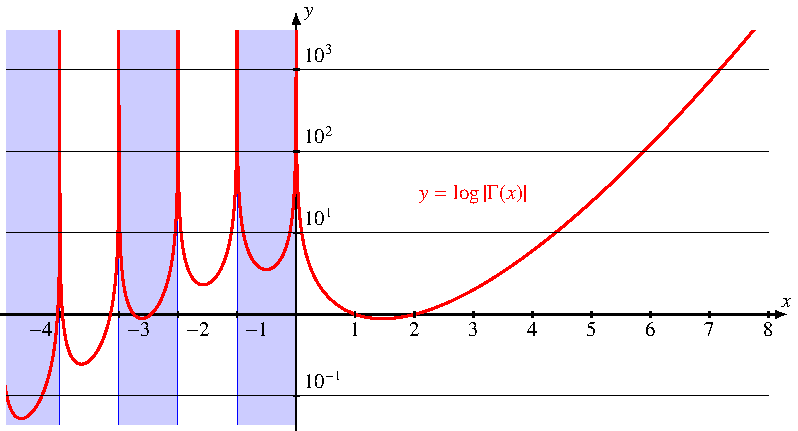
\includegraphics{chapters/040-rekursion/images/loggammaplot.pdf}
\caption{Der Graph der Funktion $\log|\Gamma(x)|$ ist für $x>0$ konvex. 
Die blau hinterlegten Bereiche zeigen an, wo die Gamma-Funktion
negative Werte annimmt.
\label{buch:rekursion:gamma:loggammaplot}}
\end{figure}
Die Integralformel und die Grenzwertdefinition für die Gamma-Funktion
zeigen beide, dass das Problem der Ausdehnung der Fakultät zu einer
Funktion $\mathbb{C}\to\mathbb{C}$ eine Lösung hat, aber es ist noch
nicht klar, in welchem Sinn dies die einzig mögliche Lösung ist.
Der Satz von Bohr-Mollerup gibt darauf eine Antwort.

Der Graph in Abbildung~\ref{buch:rekursion:gamma:loggammaplot}
zeigt, dass die Werte der Gamma-Funktion für $x>0$ so schnell
anwachsen, dass sogar die Funktion $\log|\Gamma(x)|$ konvex ist.
Der Satz von Bohr-Mollerup besagt, dass diese Eigenschaft zur
Charakterisierung der Gamma-Funktion verwendet werden kann.

\begin{satz}
\label{buch:satz:bohr-mollerup}
Eine Funktion $f\colon \mathbb{R}^+\to\mathbb{R}$ mit den Eigenschaften
\begin{enumerate}[i)]
\item $f(1)=1$,
\item $f(x+1)=xf(x)$ für alle $x\in\mathbb{R}^+$ und
\item die Funktion $\log f(t)$ ist konvex
\end{enumerate}
ist die Gamma-Funktion: $f(t)=\Gamma(t)$.
\index{Satz!von Bohr-Mollerup}%
\index{Bohr-Mollerup, Satz von}%
\end{satz}

Für den Beweis verwenden wir die folgende Eigenschaft einer konvexen
Funktion $g(x)$.
Sei
\begin{equation}
S(y,x) = \frac{g(y)-g(x)}{y-x}
\qquad\text{für $y-x$}
\end{equation}
die Steigung der Sekante zwischen den Punkten $(x,g(x))$ und $(y,g(y))$
des Graphen von $g$.
Da $g$ konvex ist, ist $S(y,x)$ eine monoton wachsende Funktion 
der beiden Variablen $x$ und $y$, solange $y>x$.

\begin{proof}[Beweis]
Wir halten zunächst fest, dass die Bedingungen i) und ii) zur Folge haben,
dass $f(n+1)=n!$ ist für alle positiven natürlichen Zahlen.
Für die Steigung einer Sekante der Funktion $g(x)=\log f(x)$ kann damit
für natürliche Argumente bereits berechnet werden, es ist
\[
S(n,n+1)
=
\frac{\log n! - \log (n-1)!}{n+1-n}
=
\frac{\log n + \log (n-1)! - \log(n-1)!}{1}
=
\log n
\]
und entsprechend auch $S(n-1,n) = \log(n-1)$.

\begin{figure}
\begin{center}
\begin{tikzpicture}[>=latex,thick]
\draw (-6,0) -- (6,0);

\node at (-5,0) [above] {$n-1\mathstrut$};
\node at (0,0) [above] {$n\mathstrut$};
\node at (3,0) [above] {$n+x\mathstrut$};
\node at (5,0) [above] {$n+1\mathstrut$};

\node[color=blue] at (-5,-2.3) {$S(n-1,n)\mathstrut$};
\node[color=red] at (-1.666,-2.3) {$S(n-1,n+x)\mathstrut$};
\node[color=darkgreen] at (1.666,-2.3) {$S(n,n+x)\mathstrut$};
\node[color=orange] at (5,-2.3) {$S(n,n+1)\mathstrut$};

\node at (-3.333,-2.3) {$<\mathstrut$};
\node at (0,-2.3) {$<\mathstrut$};
\node at (3.333,-2.3) {$<\mathstrut$};

\draw[color=blue] (-5,0) -- (-5,-2) -- (0,0);
\draw[color=red] (-5,0) -- (-1.666,-2) -- (3,0);
\draw[color=darkgreen] (0,0) -- (1.666,-2) -- (3,0);
\draw[color=orange] (0,0) -- (5,-2) -- (5,0);

\fill (-5,0) circle[radius=0.08];
\fill (0,0) circle[radius=0.08];
\fill (3,0) circle[radius=0.08];
\fill (5,0) circle[radius=0.08];

\draw[double,color=blue] (-5,-2.5) -- (-5,-3.0);
\draw[double,color=orange] (5,-2.5) -- (5,-3.0);

\node[color=blue] at (-5,-3.3) {$\log (n-1)\mathstrut$};
\node[color=orange] at (5,-3.3) {$\log (n)\mathstrut$};

\end{tikzpicture}
\end{center}
\caption{Für den Beweis des Satzes von Bohr-Mollerup wird die
Sekantensteigung $S(x,y)$ für die Argumente $n-1$, $n$, $n+x$ und $n+1$
verwendet.
\label{buch:rekursion:fig:bohr-mollerup}}
\end{figure}
Wir wenden jetzt die eben erwähnte Tatsache, dass $S(x,y)$ monoton
wachsend ist, auf die Punkte $n-1$, $n$, $n+x$ und $n+1$ wie
in Abbildung~\ref{buch:rekursion:fig:bohr-mollerup} an, wobei
$0<x<1$ ist.

Die linke Ungleichung in Abbildung~\ref{buch:rekursion:fig:bohr-mollerup}
ist
\begin{align}
\log(n-1)
&<
S(n-1,n+x)
=
\frac{\log f(n+x) -\log(n-2)!}{n+x-n+1}
\notag
\\
(x+1)\log(n-1) + \log(n-2)!
&< \log f(n+x),
\notag
\\
x\log(n-1) + \log(n-1)!
&< \log f(n+x)
\label{buch:rekursion:bohr-mollerup:eqn1}
\intertext{sie schätzt $\log f(n+x)$ nach unten ab.
Die Exponentialfunktion ist monoton wachsen, wendet man sie auf
\eqref{buch:rekursion:bohr-mollerup:eqn1} an, erhält man}
(n-1)^x (n-1)!
&<
f(n+x).
\label{buch:rekursion:bohr-mollerup:ungllinks}
\end{align}
Ganz ähnlich folgt aus der Ungleichung rechts in
Abbildung~\ref{buch:rekursion:fig:bohr-mollerup}
\begin{align}
\frac{\log f(n+x)-\log (n-1)!}{n+x-n}
&< \log n
\notag
\\
\log f(n+x) - \log(n-1)!
&<
x \log n
\notag
\\
\log f(n+x) 
&<
x\log n + \log(n-1)!
\notag
\intertext{und nach Anwendung der Exponentialfunktion}
f(n+x)
&<
n^x (n-1)!
\label{buch:rekursion:bohr-mollerup:unglrechts}
\end{align}
Die Funktion $f(n+x)$ können wir jetzt mit der Funktionalgleichung ii)
durch $f(x)$ ausdrücken:
\begin{align*}
f(n+x)
&=
(x+n-1)f(n+x-1)
\\
&=
(x+n-1)(x+n-2)f(n+x-2)
\\
&\vdots
\\
&=
(x+n-1)(x+n-2)\dots x\,f(x)
=
(x)_n f(x).
\end{align*}
Zusammen mit den Ungleichungen
\eqref{buch:rekursion:bohr-mollerup:ungllinks}
und
\eqref{buch:rekursion:bohr-mollerup:unglrechts}
erhalten wir
\begin{align*}
(n-1)^x (n-1)!
&<
(x)_n f(x)
<
n^x (n-1)!
\intertext{oder nach Division durch $(x)_n$}
%\underbrace{
\frac{(n-1)^x (n-1)!}{(x)_n}
%}_{\displaystyle\to \Gamma(x)}
&< f(x)
<
\frac{n^x (n-1)!}{(x)_n}
=
%\underbrace{
\frac{n^x n!}{(x)_{n+1}}
%}_{\displaystyle\to \Gamma(x)}
\cdot
%\underbrace{
\frac{x+n}{n}
%}_{\displaystyle\to 1}
.
\end{align*}
Der Ausdruck ganz links und der erste Bruch rechts konvergieren
für $n\to\infty$ beide gegen $\Gamma(x)$ und der Bruch ganz rechts
konvergiert gegen $1$.
Daher muss auch $f(x)=\Gamma(x)$ sein.
\end{proof}

%
% 12-integral.tex
%
% (c) 2022 Prof Dr Andreas Müller, OST Ostschweizer Hochschule
%
\subsection{Integraldarstellung und der Satz von Bohr-Mollerup
\label{buch:subsection:integral-eindeutig}}
Die Integralformel
\[
f(x)
=
\int_0^\infty t^{x-1}e^{-t}\,dt
\]
für die Gamma-Funktion erfüllt die Funktionalgleichung der Gamma-Funktion.
Aus dem Satz von Bohr-Mollerup~\ref{buch:satz:bohr-mollerup} folgt,
dass $f(x)=\Gamma(x)$, wenn gezeigt werden kann, dass $\log f(x)$
konvex ist.
Dies soll im Folgenden gezeigt werden.

\subsubsection{Logarithmische Ableitung}
\index{logarithmische Ableitung}%
Die Ableitungen der Funktion $\log f(x)$ sind die erste und
zweite logarithmische
\index{logarithmische Ableitung!zweite}%
Ableitung
\begin{align}
\frac{d}{dx}\log f(x)
&=
\frac{f'(x)}{f(x)}
\notag
\\
\frac{d^2}{dx^2} \log f(x)
&=
\frac{f''(x)f(x)-f'(x)^2}{f(x)^2}.
\label{buch:rekursion:eqn:zweiteablteitung}
\end{align}
Durch Ableiten unter dem Integralzeichen können die Ableitungen
von $f$ als
\begin{align*}
f'(x)
&=
\int_0^\infty \log(t)\, t^{x-1} e^{-t}\,dt
\\
f''(x)
&=
\int_0^\infty \log(t)^2\, t^{x-1} e^{-t}\,dt
\end{align*}
bestimmt werden.
Um nachzuweisen, dass $\log f(x)$ konvex ist, muss nur gezeigt werden,
dass die zweite logarithmische Ableitung von $f(x)$ positiv ist, was
gemäss~\eqref{buch:rekursion:eqn:zweiteablteitung} mit
\begin{equation}
f''(x)f(x)-f'(x)^2
=
\int_0^\infty \log(t)^2\, t^{x-1}e^{-t}\,dt
\int_0^\infty t^{x-1}e^{-t}\,dt
-
\biggl(
\int_0^\infty \log(t)\, t^{x-1}e^{-t}\,dt
\biggr)^2
\ge 0
\label{buch:rekursion:gamma-integral:ungleichung}
\end{equation}
gleichbedeutend ist.

\subsubsection{Skalarprodukt}
Die Integral in~\eqref{buch:rekursion:gamma-integral:ungleichung}
können als Werte eines Skalarproduktes von Funktionen auf $\mathbb{R}^+$
\index{Skalarprodukt}%
gelesen werden.
Dazu definieren wir
\begin{align}
\langle u,v\rangle
&=
\int_0^\infty u(t)v(t)\,t^{x-1}e^{-t}\,dt
\label{buch:rekursion:gamma-integral:eqn:skalarprodukt}
\\
\|u\|^2
&=
\int_0^\infty u(t)^2 \,t^{x-1}e^{-t}\,dt,
\notag
\end{align}
für alle Funktionen $u$ und $v$, für die die Integrale definiert sind.

\subsubsection{Cauchy-Schwarz-Ungleichung}
Die Cauchy-Schwarz-Ungleichung für das
Skalarprodukt~\eqref{buch:rekursion:gamma-integral:eqn:skalarprodukt}
\index{Cauchy-Schwarz-Ungleichung}
für die Funktion $u(t)=1$ und $v(t)=\log(t)$
lautet
\[
|\langle u,v\rangle|^2
=
\biggl|
\int_0^1 \log(t)\,t^{x-1}e^{-t}\,dt
\biggr|^2
\le
\|u\|^2\cdot \|v\|^2
=
\int_0^\infty 1\cdot t^{x-1}e^{-t}\,dt
\int_0^\infty \log(t)^2\cdot t^{x-1}e^{-t}\,dt.
\]
Daraus folgt aber durch Umstellen unmittelbar die
Ungleichung~\eqref{buch:rekursion:gamma-integral:ungleichung}.
Damit ist gezeigt, dass $\log f(t)$ konvex ist und nach
dem Satz~\ref{buch:satz:bohr-mollerup} folgt nun, dass $f(x)=\Gamma(x)$.




%
% Beta-Integrale
%
% (c) 2021 Prof Dr Andreas Müller, OST Ostschweizer Fachhochschule
%
\section{Die Beta-Funktion
\label{buch:rekursion:gamma:section:beta}}
Die Eulersche Integralformel für die Gamma-Funktion in
Definition~\ref{buch:rekursion:def:gamma} wurde in
Abschnitt~\ref{buch:subsection:integral-eindeutig}
mit dem Satz~\ref{buch:satz:bohr-mollerup}
von Bohr-Mollerup gerechtfertigt.
Man kann Sie aber auch als Grenzfall der Beta-Funktion verstehen,
die in diesem Abschnitt dargestellt wird.


\subsection{Beta-Integral
\label{buch:rekursion:gamma:subsection:integralbeweis}}
In diesem Abschnitt wird das Beta-Integral eingeführt, eine Funktion
von zwei Variablen, welches eine Integral-Definition mit einer
reichaltigen Menge von Rekursionsbeziehungen hat, die sich direkt auf
die Gamma-Funktion zurückführen lassen.
Daraus wird sich dann ein Beweis für die Integralformel für die
Gamma-Funktion ergeben.

\begin{definition}
\label{buch:rekursion:gamma:def:beta-funktion}
Das Beta-Integral ist das Integral
\[
B(x,y)
=
\int_0^1 t^{x-1} (1-t)^{y-1}\,dt
\]
für $\operatorname{Re}x>0$, $\operatorname{Re}y>0$.
\index{Beta-Integral}%
\end{definition}

Aus der Definition kann man sofort ablesen, dass $B(x,y)=B(y,x)$.
Für $y=1$ folgt ausserdem
\begin{equation}
B(x,1)
=
\int_0^1 t^{x-1}\,dt
=
\biggl[ \frac{t^x}{x}\biggr]_0^1
=
\frac{1}{x}.
\label{buch:rekursion:gamma:betax1}
\end{equation}
Speziell gilt $B(1,1)=1$.

\subsubsection{Rekursionsformeln für das Beta-Integral}
Aus der Definition folgt direkt
\begin{align*}
B(x,y+1)
&=
\int_0^1 t^{x-1} (1-t)^{y+1-1}\,dt
=
\int_0^1 (1-t) t^{x-1} (1-t)^{y-1}\,dt
\\
&=
\int_0^1 t^{x-1} (1-t)^{y-1}\,dt
-
\int_0^1 t^{x} (1-t)^{y-1}\,dt
\\
&=
B(x,y) - B(x+1,y)
\end{align*}
oder
\begin{equation}
B(x,y) = B(x+1,y) + B(x,y+1).
\label{buch:rekursion:gamma:betarek1}
\end{equation}
%
%XXX Vergleich mit der Rekursionsformel für Binomialkoeffizienten
%
Durch partielle Integration kann man eine weitere Rekursionsformel finden.
Dazu berechnet man
\begin{align}
B(x,y+1)
&=
\int_0^1 t^{x-1}(1-t)^{y}\,dt
\notag
\\
&=
\biggl[\frac{t^x}x(1-t)^y\biggr]_0^1
+
\frac{y}x \int_0^1 t^x(1-t)^{y-1}\,dt
\notag
\\
&=
 \frac{y}x B(x+1,y).
\label{buch:rekursion:gamma:betarek2}
\end{align}
Durch Gleichsetzen
\eqref{buch:rekursion:gamma:betarek1}
und
\eqref{buch:rekursion:gamma:betarek2}
entsteht die Rekursionsformel
\[
B(x,y)-B(x,y+1)
=
B(x+1,y)
=
\frac{x}{y}B(x,y+1)
\]
oder
\begin{equation}
B(x,y)
=
\frac{x+y}{y}B(x,y+1).
\label{buch:rekursion:gamma:betarek3}
\end{equation}

\subsubsection{Beta-Funktion und Gamma-Funktion}
Die Rekursionsbeziehung~\eqref{buch:rekursion:gamma:betarek3}
kann jetzt dazu verwendet werden, eine Darstellung der Beta-Funktion
durch die Gamma-Funktion zu finden.
Durch $n$-fache Anwendung von \eqref{buch:rekursion:gamma:betarek3}
ergibt sich zunächst
\begin{align*}
B(x,y)
&=
\frac{x+y}{y}
B(x,y+1)
=
\frac{x+y}{y}
\frac{x+y+1}{y+1}
B(x,y+2)
\\
&=
\frac{x+y}{y}
\frac{x+y+1}{y+1}
\cdot
\ldots
\cdot
\frac{x+y+n-1}{y+n-1}
B(x,y+n)
=
\frac{(x+y)_n}{(y)_n}
B(x,y+n)
\intertext{Die Beta-Funktion auf der rechten Seite kann als Integral
geschrieben werden:}
&=
\frac{(x+y)_n}{(y)_n}
\int_0^1 t^{x-1}(1-t)^{y+n-1}\,dt.
\end{align*}
Wir halten dieses Zwischenresultat für spätere Verwendung fest.

\begin{lemma}
\label{buch:rekursion:gamma:betareklemma}
Für $n\in\mathbb{N}$ gilt
\[
B(x,y+n) = \frac{(y)_n}{(x+y)_n} B(x,y).
\]
\end{lemma}

Wir streben an, mit dem Grenzübergang $n\to\infty$ aus den
Pochhammer-Symbolen Gamma-Funktionen zu machen, dazu müssen gemäss
Definition~\ref{buch:rekursion:gamma:def:definition} weitere Faktoren
$1/(n!\,n^{x-1})$ vorhanden sein.
Wir erweitern geeignet und nehmen die übrig bleibenden Faktoren in
das Integral.
So ergibt sich
\begin{align}
B(x,y)
&=
\frac{(x+y)_n}{n!\, n^{x+y-1}}
\frac{n!\,n^{y-1}}{(y)_n}
\int_0^1 n^{x} t^{x-1}(1-t)^{y+n-1}\,dt.
\notag
\intertext{Mit der Substition $s/n=t$ wird das Integral zu einem Integral
über das Interval $[0,n]$}
&=
\frac{(x+y)_n}{n!\, n^{x+y-1}}
\frac{n!\,n^{y-1}}{(y)_n}
\int_0^n
n^{x}
\biggl(\frac{s}{n}\biggr)^{x-1}
\biggl(1-\frac{s}{n}\biggr)^{y+n-1}
\,\frac{ds}{n}.
\notag
\\
&=
\frac{(x+y)_n}{n!\, n^{x+y-1}}
\frac{n!\,n^{y-1}}{(y)_n}
\int_0^n
n^{x-1}
\biggl(\frac{s}{n}\biggr)^{x-1}
\biggl(1-\frac{s}{n}\biggr)^{y+n-1}
\,ds.
\intertext{Beim Grenzübergang $n\to\infty$ wird daraus}
&=
\underbrace{\frac{(x+y)_n}{n!\, n^{x+y-1}}}_{\displaystyle \to 1/\Gamma(x+y)}
\underbrace{\frac{n!\,n^{y-1}}{(y)_n}}_{\displaystyle\to \Gamma(y)}
\int_0^n
s^{x-1}
\underbrace{\biggl(1-\frac{s}{n}\biggr)^{n}}_{\displaystyle\to e^{-s}}
\underbrace{\biggl(1-\frac{s}{n}\biggr)^{y-1}}_{\displaystyle\to 1}
\,ds.
\notag
\\
&\to \frac{\Gamma(y)}{\Gamma(x+y)} \int_0^\infty s^{x-1}e^{-s}\,ds.
\label{buch:rekursion:gamma:betagamma}
\end{align}
Das Integral im letzten Ausdruck ist die Integraldarstellung für 
die Gamma-Funktion von Definition~\ref{buch:rekursion:def:gamma},
die bis anhin noch nicht gerechtfertigt wurde.

In~\eqref{buch:rekursion:gamma:betax1} ist gezeigt worden, dass
$B(x,1)=1/x$.
Andererseits zeigt \eqref{buch:rekursion:gamma:betagamma} für $y=1$,
dass
\begin{align}
\frac1x
=
B(x,1)
&= 
\frac{\Gamma(1)}{\Gamma(x+1)}\int_0^\infty s^{x-1}e^{-s}\,ds.
\notag
\intertext{%
Wegen $\Gamma(1)=1$ und $\Gamma(x+1)=x\Gamma(x)$ finden wir nach
Multiplikation mit $x\Gamma(x)$:}
\Gamma(x)
&=
\int_0^\infty s^{x-1}e^{-s}\,ds,
\label{buch:rekursion:gamma:integralbeweis}
\end{align}
was die Integraldarstellung
von Definition~\ref{buch:rekursion:def:gamma},
der Gamma-Funktion beweist.
Durch Einsetzen der Integralformel im Ausdruck
\eqref{buch:rekursion:gamma:betagamma} folgt der folgende
Satz.

\begin{satz}
\index{Satz!Beta-Funktion und Gamma-Funktion}%
Die Beta-Funktion kann aus der Gamma-Funktion nach
\begin{equation}
B(x,y) = \frac{\Gamma(x)\Gamma(y)}{\Gamma(x+y)}
\label{buch:rekursion:gamma:betagamma}
\end{equation}
berechnet werden.
\end{satz}

%
% Info über die Beta-Verteilung
%
%
% teil1.tex -- Beispiel-File für das Paper
%
% (c) 2020 Prof Dr Andreas Müller, Hochschule Rapperswil
%
\subsection{Ordnungsstatistik und Beta-Funktion
\label{buch:rekursion:ordnung:section:ordnungsstatistik}}
\rhead{Ordnungsstatistik und Beta-Funktion}
In diesem Abschnitt ist $X$ eine Zufallsvariable mit der Verteilungsfunktion
$F_X(x)$, und $X_i$, $1\le i\le n$ sei ein Stichprobe von unabhängigen
Zufallsvariablen, die wie $X$ verteilt sind.
Ziel ist, die Verteilungsfunktion und die Wahrscheinlichkeitsdichte
des grössten, zweitgrössten, $k$-t-grössten Wertes in der Stichprobe
zu finden.
Wir schreiben $[n]=\{1,\dots,n\}$ für die Menge der natürlichen
Zahlen von zwischen $1$ und $n$.

\subsubsection{Verteilung von $\operatorname{max}(X_1,\dots,X_n)$ und
$\operatorname{min}(X_1,\dots,X_n)$
\label{buch:rekursion:ordnung:subsection:minmax}}
Die Verteilungsfunktion von $\operatorname{max}(X_1,\dots,X_n)$ hat
den Wert
\begin{align*}
F_{\operatorname{max}(X_1,\dots,X_n)}(x)
&=
P(\operatorname{max}(X_1,\dots,X_n) \le x)
\\
&=
P(X_1\le x\wedge \dots \wedge X_n\le x)
\\
&=
P(X_1\le x) \cdot \ldots \cdot P(X_n\le x)
\\
&=
P(X\le x)^n
=
F_X(x)^n.
\end{align*}
Für die Gleichverteilung ist
\[
F_{\text{equi}}(x)
=
\begin{cases}
0&\qquad x< 0
\\
x&\qquad 0\le x\le 1
\\
1&\qquad 1<x.
\end{cases}
\]
In diesem Fall ist Verteilung des Maximums
\[
F_{\operatorname{max}(X_1,\dots,X_n)}(x)
=
\begin{cases}
0&\qquad x<0\\
x^n&\qquad 0\le x\le 1\\
1&\qquad 1 < x.
\end{cases}
\]
Mit der zugehörigen Wahrscheinlichkeitsdichte
\[
\varphi_{\operatorname{max}(X_1,\dots,X_n)}
=
\frac{d}{dx}
F_{\operatorname{max}(X_1,\dots,X_n)}(x)
=
\begin{cases}
nx^{n-1}&\qquad 0\le x\le 1\\
0       &\qquad \text{sonst}
\end{cases}
\]
kann man zum Beispiel den Erwartungswert
\[
E(\operatorname{max}(X_1,\dots,X_n))
=
\int_{-\infty}^\infty 
x
\varphi_{\operatorname{X_1,\dots,X_n}}(x)
\,dx
=
\int_{0}^1 x\cdot nx^{n-1}\,dt
=
\biggl[
\frac{n}{n+1}x^{n+1}
\biggr]_0^1
=
\frac{n}{n+1}
\]
berechnen.

Ganz analog kann man auch die Verteilungsfunktion von
$\operatorname{min}(X_1,\dots,X_n)$ bestimmen.
Sie ist
\begin{align*}
F_{\operatorname{min}(X_1,\dots,X_n)}(x)
&=
P(x\le X_1\vee \dots \vee x\le X_n)
\\
&=
1-
P(x > X_1\wedge \dots \wedge x > X_n)
\\
&=
1-
(1-P(x\le X_1)) \cdot\ldots\cdot (1-P(x\le X_n))
\\
&=
1-(1-F_X(x))^n,
\end{align*}
Im Speziellen für im Intervall $[0,1]$ gleichverteilte $X_i$ ist die
Verteilungsfunktion des Minimums
\[
F_{\operatorname{min}(X_1,\dots,X_n)}(x)
=
\begin{cases}
0        &\qquad x<0        \\
1-(1-x)^n&\qquad 0\le x\le 1\\
1        &\qquad 1 < x
\end{cases}
\]
mit Wahrscheinlichkeitsdichte
\[
\varphi_{\operatorname{min}(X_1,\dots,X_n)}
=
\frac{d}{dx}
F_{\operatorname{min}(X_1,\dots,X_n)}
=
\begin{cases}
n(1-x)^{n-1}&\qquad 0\le x\le 1\\
0           &\qquad \text{sonst}
\end{cases}
\]
und Erwartungswert
\begin{align*}
E(\operatorname{min}(X_1,\dots,X_n)
&=
\int_{-\infty}^\infty x\varphi_{\operatorname{min}(X_1,\dots,X_n)}(x)\,dx
=
\int_0^1 x\cdot n(1-x)^{n-1}\,dx
\\
&=
\bigl[ -x(1-x)^n \bigr]_0^1 + \int_0^1 (1-x)^n\,dx
=
\biggl[
-
\frac{1}{n+1}
(1-x)^{n+1}
\biggr]_0^1
=
\frac{1}{n+1}.
\end{align*}
Es ergibt sich daraus als natürlich Verallgemeinerung die Frage nach
der Verteilung des zweitegrössten oder zweitkleinsten Wertes unter den
Werten $X_i$.

\subsubsection{Der $k$-t-grösste Wert}
Sie wieder $X_i$ eine Stichprobe von $n$ unabhängigen wie $X$ verteilten
Zufallsvariablen.
Diese werden jetzt der Grösse nach sortiert, die sortierten Werte werden
mit
\[
X_{1:n} \le X_{2:n} \le \dots \le X_{(n-1):n} \le X_{n:n}
\]
bezeichnet.
Die Grössen $X_{k:n}$ sind Zufallsvariablen, sie heissen die $k$-ten
Ordnungsstatistiken.
Die in Abschnitt~\ref{buch:rekursion:ordnung:subsection:minmax} behandelten Zufallsvariablen
$\operatorname{min}(X_1,\dots,X_n)$
und
$\operatorname{max}(X_1,\dots,X_n)$
sind die Fälle
\begin{align*}
X_{1:n} &= \operatorname{min}(X_1,\dots,X_n) \\
X_{n:n} &= \operatorname{max}(X_1,\dots,X_n).
\end{align*}

Um den Wert der Verteilungsfunktion von $X_{k:n}$ zu berechnen, müssen wir 
die Wahrscheinlichkeit bestimmen, dass $k$ der $n$ Werte $X_i$ $x$ nicht
übersteigen.
Der $k$-te Wert $X_{k:n}$ übersteigt genau dann $x$ nicht, wenn
mindestens $k$ der Zufallswerte $X_i$ $x$ nicht übersteigen, also
\[
P(X_{k:n} \le x)
=
P\left(
|\{i\in[n]\,|\, X_i\le x\}| \ge k
\right).
\]

Das Ereignis $\{X_i\le x\}$ ist eine Bernoulli-Experiment, welches mit
Wahrscheinlichkeit $F_X(x)$ eintritt.
Die Anzahl der Zufallsvariablen $X_i$, die $x$ übertreffen, ist also
Binomialverteilt mit $p=F_X(x)$.
Damit haben wir gefunden, dass mit Wahrscheinlichkeit
\begin{equation}
F_{X_{k:n}}(x)
=
P(X_{k:n}\le x)
=
\sum_{i=k}^n \binom{n}{i}F_X(x)^i (1-F_X(x))^{n-i}
\label{buch:rekursion:ordnung:eqn:FXkn}
\end{equation}
mindestens $k$ der Zufallsvariablen den Wert $x$ überschreiten.

\subsubsection{Wahrscheinlichkeitsdichte der Ordnungsstatistik}
Die Wahrscheinlichkeitsdichte der Ordnungsstatistik kann durch Ableitung
von \eqref{buch:rekursion:ordnung:eqn:FXkn} gefunden, werden, sie ist
\begin{align*}
\varphi_{X_{k:n}}(x)
&=
\frac{d}{dx}
F_{X_{k:n}}(x)
\\
&=
\sum_{i=k}^n
\binom{n}{i}
\bigl(
iF_X(x)^{i-1}\varphi_X(x) (1-F_X(x))^{n-i}
-
F_X(x)^k
(n-i)
(1-F_X(x))^{n-i-1}
\varphi_X(x)
\bigr)
\\
&=
\sum_{i=k}^n
\binom{n}{i}
\varphi_X(x)
F_X(x)^{i-1}(1-F_X(x))^{n-i-1}
\bigl(
iF_X(x)-(n-i)(1-F_X(x))
\bigr)
\\
&=
\varphi_X(x)
\biggl(
\sum_{i=k}^n i\binom{n}{i} F_X(x)^{i-1}(1-F_X(x))^{n-i}
-
\sum_{j=k}^n (n-j)\binom{n}{j} F_X(x)^{j}(1-F_X(x))^{n-j-1}
\biggr)
\\
&=
\varphi_X(x)
\biggl(
\sum_{i=k}^n i\binom{n}{i} F_X(x)^{i-1}(1-F_X(x))^{n-i}
-
\sum_{i=k+1}^{n+1} (n-i+1)\binom{n}{i-1} F_X(x)^{i-1}(1-F_X(x))^{n-i}
\biggr)
\\
&=
\varphi_X(x)
\biggl(
k\binom{n}{k}F_X(x)^{k-1}(1-F_X(x))^{n-k}
+
\sum_{i=k+1}^{n+1}
\left(
i\binom{n}{i} 
-
(n-i+1)\binom{n}{i-1}
\right)
F_X(x)^{i-1}(1-F_X(x))^{n-i}
\biggr)
\end{align*}
Mit den wohlbekannten Identitäten für die Binomialkoeffizienten
\begin{align*}
i\binom{n}{i} 
-
(n-i+1)\binom{n}{i-1}
&=
n\binom{n-1}{i-1}
-
n
\binom{n-1}{i-1}
=
0
\end{align*}
folgt jetzt
\begin{align*}
\varphi_{X_{k:n}}(x)
&=
\varphi_X(x)k\binom{n}{k} F_X(x)^{k-1}(1-F_X(x))^{n-k}.
\intertext{Im Speziellen für gleichverteilte Zufallsvariablen $X_i$ ist
}
\varphi_{X_{k:n}}(x)
&=
k\binom{n}{k} x^{k-1}(1-x)^{n-k}.
\end{align*}
Dies ist die Wahrscheinlichkeitsdichte einer Betaverteilung
\[
\beta(k,n-k+1)(x)
=
\frac{1}{B(k,n-k+1)}
x^{k-1}(1-x)^{n-k}.
\]
Tatsächlich ist die Normierungskonstante 
\begin{align}
\frac{1}{B(k,n-k+1)}
&=
\frac{\Gamma(n+1)}{\Gamma(k)\Gamma(n-k+1)}
=
\frac{n!}{(k-1)!(n-k)!}.
\label{buch:rekursion:ordnung:betaverteilung:normierung1}
\end{align}
Andererseits ist
\[
k\binom{n}{k}
=
k\frac{n!}{k!(n-k)!}
=
\frac{n!}{(k-1)!(n-k)!},
\]
in Übereinstimmung mit~\eqref{buch:rekursion:ordnung:betaverteilung:normierung1}.
Die Verteilungsfunktion und die Wahrscheinlichkeitsdichte der
Ordnungsstatistik sind in Abbildung~\ref{buch:rekursion:ordnung:fig:order} dargestellt.

\begin{figure}
\centering
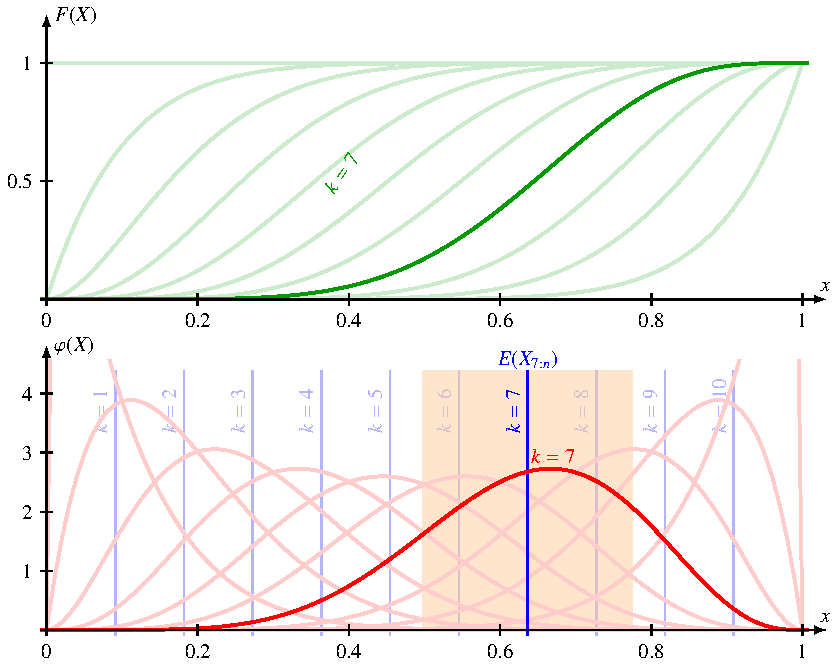
\includegraphics{chapters/040-rekursion/images/order.pdf}
\caption{Verteilungsfunktion und Wahrscheinlichkeitsdichte der
Ordnungsstatistiken $X_{k:n}$ einer gleichverteilung Zuvallsvariable
mit $n=10$.
\label{buch:rekursion:ordnung:fig:order}}
\end{figure}

%
% Die Beta-Funktion
%
\subsection{Die Beta-Verteilung
\label{buch:rekursion:subsection:beta-verteilung}}
Die Wahrscheinlichkeitsdichte, die im
Abschnitt~\ref{buch:rekursion:ordnung:section:ordnungsstatistik}
gefunden worden ist, ist nicht nur für ganzzahlige Exponenten
definiert.

\begin{figure}
\centering
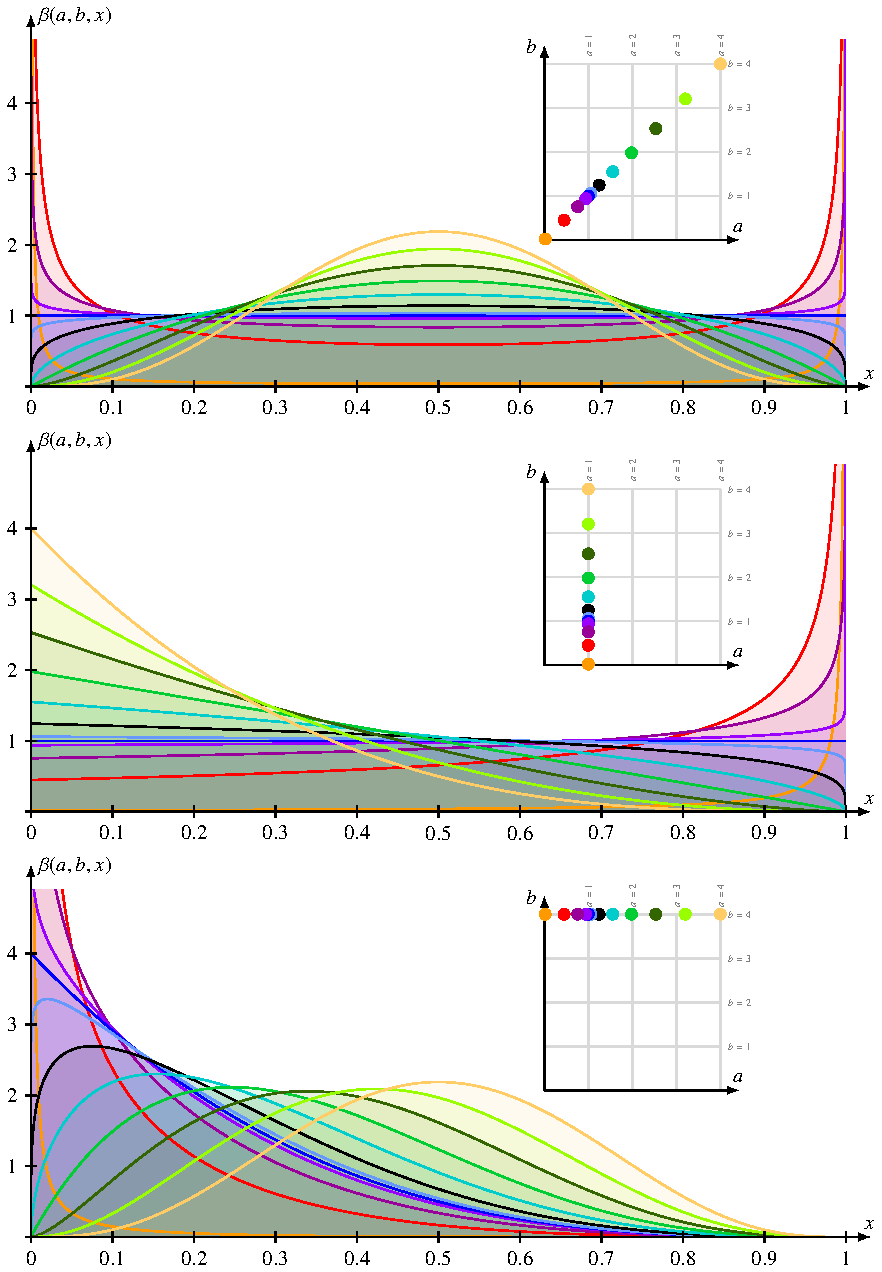
\includegraphics[width=0.92\textwidth]{chapters/040-rekursion/images/beta.pdf}
\caption{Wahrscheinlichkeitsdichte der Beta-Verteilung
$\beta(a,b,x)$
für verschiedene Werte der Parameter $a$ und $b$.
Die Werte des Parameters für einen Graphen einer Beta-Verteilung
sind im kleinen Quadrat rechts im Graphen
als Punkt mit der gleichen Farbe dargestellt.
\label{buch:rekursion:ordnung:fig:betaverteilungn}}
\end{figure}

\begin{definition}
Die Beta-Verteilung ist die Verteilung mit der Wahrscheinlichkeitsdichte
\[
\beta_{a,b}(x)
=
\begin{cases}
\displaystyle
\frac{1}{B(a,b)}
x^{a-1}(1-x)^{b-1}&\qquad 0\le x \le 1\\
0&\qquad\text{sonst.}
\end{cases}
\]
\end{definition}

Die Beta-Funktion ist also die Normierungskonstante der Beta-Verteilung.
Die wichtigsten Kennzahlen der Beta-Verteilung wie Erwartungswert und
Varianz lassen sich alle ebenfalls als Werte der Beta-Funktion ausdrücken.

\subsubsection{Erwartungswert}
Mit der Wahrscheinlichkeitsdichte kann man jetzt auch den Erwartungswerte
der $k$-ten Ordnungsstatistik bestimmen.
Die Rechnung ergibt:
\begin{align*}
E(X_{k:n})
&=
\int_0^1 x\cdot k\binom{n}{k} x^{k-1}(1-x)^{n-k}\,dx
=
k
\binom{n}{k}
\int_0^1
x^{k}(1-x)^{n-k}\,dx.
\intertext{Dies ist das Beta-Integral}
&=
k\binom{n}{k}
B(k+1,n-k+1)
\intertext{welches man durch Gamma-Funktionen bzw.~durch Fakultäten wie in}
&=
k\frac{n!}{k!(n-k)!}
\frac{\Gamma(k+1)\Gamma(n-k+1)}{n+2}
=
k\frac{n!}{k!(n-k)!}
\frac{k!(n-k)!}{(n+1)!}
=
\frac{k}{n+1}
\end{align*}
ausdrücken kann.
Die Erwartungswerte haben also regelmässige Abstände, sie sind in
Abbildung~\ref{buch:rekursion:ordnung:fig:order} als blaue vertikale Linien eingezeichnet.

Für die Beta-Verteilung lässt sich die Rechnung noch allgemeiner 
durchführen.
Der Erwartungswert einer $\beta_{a,b}$-verteilten Zufallsvariablen $X$
ist
\begin{align*}
E(X)
&=
\int_0^1 x \beta_{a,b}(x)\,dx
=
\frac{1}{B(a,b)}
\int_0^1 x\cdot x^{a-1}(1-x)^{b-1}\,dx
=
\frac{B(a+1,b)}{B(a,b)}
=
\frac{a}{a+b}.
\end{align*}
Durch Einsetzen von $a=k+1$ und $b=n-k+1$ lassen sich die für die
Ordnungsstatistik berechneten Werte wiederfinden.

\subsubsection{Varianz}
Auch die Varianz lässt sich einfach berechnen, dazu muss zunächst
der Erwartungswert von $X_{k:n}^2$ bestimmt werden.
Er ist
\begin{align*}
E(X_{k:n}^2)
&=
\int_0^1 x^2\cdot k\binom{n}{k} x^{k-1}(1-x)^{n-k}\,dx
=
k
\binom{n}{k}
\int_0^1
x^{k+1}(1-x)^{n-k}\,dx.
\intertext{Auch dies ist ein Beta-Integral, nämlich}
&=
k\binom{n}{k}
B(k+2,n-k+1)
=
k\frac{n!}{k!(n-k)!}
\frac{(k+1)!(n-k)!}{(n+2)!}
=
\frac{k(k+1)}{(n+1)(n+2)}.
\end{align*}
Die Varianz wird damit
\begin{align}
\operatorname{var}(X_{k:n})
&=
E(X_{k:n}^2) - E(X_{k:n})^2
\notag
\\
&
=
\frac{k(k+1)}{(n+1)(n+2)}-\frac{k^2}{(n+1)^2}
=
\frac{k(k+1)(n+1)-k^2(n+2)}{(n+1)^2(n+2)}
=
\frac{k(n-k+1)}{(n+1)^2(n+2)}.
\label{buch:rekursion:ordnung:eqn:ordnungsstatistik:varianz}
\end{align}
In Abbildung~\ref{buch:rekursion:ordnung:fig:order} ist die Varianz der
Ordnungsstatistik $X_{k:n}$ für $k=7$ und $n=10$ als oranges
Rechteck dargestellt.

Auch die Varianz kann ganz allgemein für die Beta-Verteilung
bestimmt werden.
Dazu berechnen wir zunächst
\begin{align*}
E(X^2)
&=
\frac{1}{B(a,b)}
\int_0^1
x^2\cdot x^{a-1}(1-y)^{b-1}\,dx
=
\frac{B(a+2,b)}{B(a,b)}.
\end{align*}
Daraus folgt dann 
\[
\operatorname{var}(X)
=
E(X^2)-E(X)^2
=
\frac{B(a+2,b)B(a,b)-B(a+1,b)^2}{B(a,b)^2}.
\]

Die Formel~\eqref{buch:rekursion:ordnung:eqn:ordnungsstatistik:varianz}
besagt auch, dass die Varianz der proportional ist zu $k((n+1)-k)$.
Dieser Ausdruck ist am grössten für $k=(n+1)/2$, die Varianz ist
also grösser für die ``mittleren'' Ordnungstatistiken als für die
extremen $X_{1:n}=\operatorname{min}(X_1,\dots,X_n)$ und
$X_{n:n}=\operatorname{max}(X_1,\dots,X_n)$.



\subsection{Weitere Eigenschaften der Gamma-Funktion}
Die nahe Verwandtschaft der Gamma- mit der Beta-Funktion ermöglicht
nun, weitere Eigenschaften der Gamma-Funktion mit Hilfe der Beta-Funktion
herzuleiten.

\subsubsection{Nochmals der Wert von $\Gamma(\frac12)$?}
Der Wert von $\Gamma(\frac12)=\sqrt{\pi}$ wurde bereits in
\eqref{buch:rekursion:gamma:wert12}
direkt mit Hilfe der Integraldefinition berechnet.
Hier wird eine alternative Berechnungsmöglichkeit mit Hilfe der
Beta-Funktion vorgestellt.

Als Anwendung der Formel~\eqref{buch:rekursion:gamma:betagamma}
untersuchen wir den Fall $y=1-x$.
In diesem Fall wird der Nenner zu $\Gamma(x+1-x)=\Gamma(1)=1$ und damit
\begin{equation}
\Gamma(x)\Gamma(1-x)
=
B(x,1-x) 
=
\int_0^1 t^{x-1}(1-t)^{-x}\,dt.
\label{buch:rekursion:gamma:spiegelung-betaintegral}
\end{equation}
Sofern man in der Lage ist, das Integral auf der rechten Seite von
\eqref{buch:rekursion:gamma:spiegelung-betaintegral} auszuwerten,
kann man eine einfache Beziehung zwischen zwei Werten der Gamma-Funktion
an Stellen, die durch eine Spiegelung an der Geraden
$\operatorname{Re}x=\frac12$ auseinander hervorgehen.
Für $x=\frac12$ wird der Ausdruck besonders einfach:
\[
\Gamma({\textstyle\frac12})^2
=
\int_0^1 t^{-\frac12}(1-t)^{-\frac12}\,dt
=
\int_0^1 \frac{1}{\sqrt{t(1-t)\mathstrut}}\,dt.
\]
Mit der Substition $t=\sin^2 s$ wird daraus
\[
\int_0^{\frac{\pi}2}
\frac{1}{
\sqrt{\sin^2s(1-\sin^2s)}
}
2\sin s\cos s
\,ds
=
2
\int_0^{\frac{\pi}2}
\,ds
=
\pi,
\]
wobei wir $dt = 2\sin s\cos s\,ds$ verwendet haben.
Somit folgt
\begin{equation}
\Gamma({\textstyle\frac12})^2 = \pi
\qquad\Rightarrow\qquad
\Gamma({\textstyle\frac12}) = \sqrt{\pi}.
\label{buch:rekursion:gamma:gamma12}
\end{equation}
Matt Parker hat auf seinem Youtube-Kanal {\em Stand-up Maths} dieses Resultat
sogar zum Titel eines Videos\footnote{\url{https://youtu.be/dGnIJFzkLI4}}
gemacht:
{\em What is the factorial of $-\nicefrac{1}{2}$?}
Die Antwort ist natürlich nur möglich, indem man
$(-\frac12)!$ als Wert
\[
(-{\textstyle\frac12})!
=
\Gamma(-{\textstyle\frac12}+1)
=
\Gamma({\textstyle\frac12})
=
\sqrt{\pi}
\]
der Gamma-Funktion interpretiert.

%
% Alternative Parametrisierung
%
\subsubsection{Alternative Parametrisierungen}
Die Substitution $t=\sin^2 s$ hat im vorangegangenen Abschnitt
ermöglicht, $\Gamma(\frac12)$ zu ermitteln.
Die Substition erlaubt aber auch, das Beta-Integral in eine alternative
Form zu bringen.
Aus der Definition~\ref{buch:rekursion:gamma:def:beta-funktion}
wird damit
\begin{align*}
B(x,y)
&=
\int_0^1 t^{x-1} (1-t)^{y-1}\,dt
\\
&=
2
\int_0^{\frac{\pi}2} \sin^{2(x-1)} s\cdot (1-\sin^2 s)^{y-1}
\cdot \sin s\cos s\,ds
\\
&=
2
\int_0^{\frac{\pi}2} \sin^{2x-1}s \cos^{2y-1} s\,ds.
\intertext{Unter Verwendung der Formel~\eqref{buch:rekursion:gamma:betagamma},
die die Beta-Funktion durch Gamma-Funktionen auszudrücken erlaubt, findet
man die Formel}
\int_0^{\frac{\pi}2} \sin^{2x-1}s \cos^{2y-1} s\,ds
&=
\frac{\Gamma(x)\Gamma(y)}{2\Gamma(x+y)}
\end{align*}
für ein bestimmtes Integral von Potenzen von Sinus- und Kosinus-Funktionen.

Die alternative Substitution $t = s/(s+1)$ verwandelt das Beta-Integral
$B(x,y)$ in ein Integral über die positive Halbachse ab:
\begin{align}
B(x,y)
&=
\int_0^1 t^{x-1}(1-t)^{y-1}\,dt
\notag
\\
&=
\int_0^\infty
\frac{s^{x-1}}{(s+1)^{x-1}}
\frac{1}{(s+1)^{y-1}}
\frac{ds}{(s+1)^2}
\notag
\\
&=
\int_0^\infty
\frac{s^{x-1}}{(s+1)^{x+y}}\,ds,
\label{buch:rekursion:gamma:beta:sinf}
\end{align}
wobei wir
\[
\frac{dt}{ds}
=
\frac{d}{ds}
\frac{s}{s+1}
=
\frac{(s+1)-s}{(s+1)^2}
=
\frac{1}{(s+1)^2}
\]
verwendet haben.
Diese Darstellung des Beta-Integrals wird später
in Satz~\ref{buch:funktionentheorie:satz:spiegelungsformel}
dazu verwendet, die Spiegelungsformel für die Gamma-Funktion
\index{Gamma-Funktion!Spiegelungsformel}%
\index{Spiegelungsformel der Gamma-Funktion}%
herzuleiten.

Eine weitere mögliche Parametrisierung verwendet $t = (1+s)/2$
mit $dt=\frac12 ds$.
Damit wird das Beta-Integral
\begin{equation}
B(x,y)
=
\int_0^1 t^{x-1}(1-t)^{y-1}\,dt
=
\frac12
\int_{-1}^1
\biggl(\frac{1+s}2\biggr)^{x-1}
\biggl(\frac{1-s}2\biggr)^{y-1}
\,ds
=
2^{1-x-y}
\int_{-1}^1
(1+s)^{x-1}(1-s)^{y-1}
\,ds.
\label{buch:rekursion:gamma:beta:symm}
\end{equation}

%
%
%
\subsubsection{Die Verdoppelungsformel von Legendre}
Die trigonometrische Substitution kann dazu verwendet werden, die
Legendresche Verdoppelungsformel für die Gamma-Funktion herzuleiten.

\begin{satz}[Legendre]
\index{Satz!Verdoppelungsformel@Verdoppelungsformel für $\Gamma(x)$}%
\[
\Gamma(x)\Gamma(x+{\textstyle\frac12})
=
2^{1-2x}\sqrt{\pi}
\Gamma(2x)
\]
\index{Verdoppelungsformel}%
\index{Gamma-Funktion!Verdoppelungsformel von Legendre}%
\end{satz}

\begin{proof}[Beweis]
Der Wert $\Gamma(2x)$ entsteht, wenn man $B(x,x)$ mit Hilfe der
Gamma-Funktion als
\[
B(x,x)
=
\frac{\Gamma(x)^2}{\Gamma(2x)}
\]
schreibt.
Das Ziel ist, $B(x,x)$ auf einem alternativen Weg zu berechnen.

Mit Hilfe von \eqref{buch:rekursion:gamma:beta:symm}
kann man das Beta-Integral zu
\begin{align*}
B(x,x)
&=
2^{1-2x}
\int_{-1}^1
(1+s)^{x-1}(1-s)^{x-1}
\,ds
=
2^{1-2x}
\int_{-1}^1(1-s^2)^{x-1}\,ds
\end{align*}
vereinfachen.
Der Integrand ist gerade, es folgt
\[
B(x,x)
=
2^{1-2x}
\cdot 2
\int_0^1(1-s^2)^{x-1}\,ds.
\]
Das Integral kann mit der Substitution $s^2=t$ wieder in die Form
eines Beta-Integrals gebracht werden:
\begin{align*}
2\int_0^1(1-s^2)^{x-1}\,ds
&=
\int_0^1 (1-t)^{x-1} \,\frac{dt}{\sqrt{t}}
=
\int_0^1 t^{\frac12-1}(1-t)^{x-1}\,dt
=
B({\textstyle\frac12},x).
\end{align*}
In der Substitution haben wir $2s\,ds = dt$ oder $2\,ds = dt/\sqrt{t}$
verwendet.
Das letzte Beta-Integral kann man nun wieder mit Gamma-Funktionen
schreiben, nämlich als
\[
B({\textstyle\frac12},x)
=
\frac{\Gamma({\textstyle\frac12})\Gamma(x)}{\Gamma(x+{\textstyle\frac12})}.
\]
Setzt man alles zusammen, erhält man jetzt
\begin{align*}
\frac{\Gamma(x)^2}{\Gamma(2x)}
&=
\frac1{2^{2x-1}}
\frac{\Gamma({\textstyle\frac12})\Gamma(x)}{\Gamma(x+{\textstyle\frac12})}
\\
\Rightarrow\qquad
\Gamma(x)\Gamma(x+{\textstyle\frac12})
&=
2^{1-2x}
\Gamma({\textstyle\frac12})\Gamma(2x)
=
2^{1-2x}\sqrt{\pi}\Gamma(2x),
\end{align*}
wobei wir den bekannten Wert $\Gamma(\frac12)=\sqrt{\pi}$ verwendet haben.
\end{proof}

Setzt man $x=\frac12$ in die Verdoppelungsformel ein, erhält man
\[
\Gamma({\textstyle\frac12})\Gamma(1) = 2^{1-2\frac12}\sqrt{\pi}\Gamma(1)
\qquad\Rightarrow\qquad
\Gamma({\textstyle\frac12}) = \sqrt{\pi},
\]
in Übereinstimmung mit dem aus \eqref{buch:rekursion:gamma:gamma12}
bereits bekannten Wert.


%
% 3-linear.tex
%
% (c) 2021 Prof Dr Andreas Müller, OST Ostschweizer Fachhochschule
%
\section{Lineare Rekursionsgleichung mit konstanten Koeffizienten
\label{buch:rekursion:section:linear}}
\kopfrechts{Lineare Rekursionsgleichungen}
Die Funktionalgleichung der Gamma-Funktion, die im
Abschnitt~\ref{buch:rekursion:section:gamma} untersucht wurde,
hat die Form einer linearen Rekursionsgleichung
\[
\Gamma(x+1) = x\Gamma(x),\qquad \Gamma(1) = 1.
\]
Gleichungen, die Werte einer Funktion für verschiedene
Argument in Beziehung setzen, heissen {\em Funktionalgleichungen}.
\index{Funktionalgleichung}%
Es war überraschend schwierig, eine Lösung für Funktionalgleichung
der Gamma-Funktion für beliebige komplexe $x$ zu finden.
In diesem Abschnitt soll daher eine Klasse von Rekursionsgleichungen
näher untersucht werden, für die einfache Lösungen möglich sind.

%
% Lineare Differenzengleichungen
%
\subsection{Lineare Differenzengleichungen}
Die Fibonacci-Zahlen sind definiert durch die lineare Rekursionsgleichung
\begin{equation}
F_{n+1\mathstrut} = F_{n\mathstrut} + F_{n-1\mathstrut},
\qquad
F_1=1,\quad F_0=0.
\label{buch:rekursion:eqn:fibonacci}
\end{equation}
\index{Fibonacci-Zahlen}%
Ganz ähnlich wie bei der Gamma-Funktion kann man auch hier die Frage
stellen, ob es eine Funktion $F(z)$ von komplexen Argument gibt derart,
dass
\begin{equation}
F(z+1) = F(z) + F(z-1), \qquad F(1)=1,\quad F(0)=0.
\label{buch:rekursion:eqn:fibonaccikomplex}
\end{equation}
\index{Fibonacci-Zahlen!komplexe}

\begin{aufgabe}
Gibt es eine Funktion
\[
F(z) = \sum_{k=0}^\infty a_k (z-z_0)^k
\]
derart, dass
\[
F(z+1) = F(z)+F(z-1)?
\]
\end{aufgabe}

Sind $F_1(z)$ und $F_2(z)$ Lösungen der Differenzengleichung, dann
sind beliebige Linearkombinationen $\lambda F_1(z) + \mu F_2(z)$
ebenfalls Lösungen.
Ausserdem ist $e^{2k\pi i}F(z)$ eine Lösung der Differenzengleichung,
es gibt also unendlich viele linear unabhängige Lösungen.

%
% Lösung mit Exponentialfunktionen
%
\subsection{Lösung mit Exponentialfunktionen}
Gesucht ist eine ganze Funktion, also eine Funktion
$F\colon\mathbb{C}\to\mathbb{C}$, die Lösung einer
Differenzengleichung
\index{Differenzengleichung}%
\begin{equation}
\sum_{k=0}^n a_kF(z+n)=0,
\end{equation}
mit $a_n\ne 1$.
ist.
Ein erfolgversprechender Ansatz ist $F(z)=e^{bz}=(e^b)^z$, da die
Exponentialfunktion eine ganze Funktion ist.
Die Differenzengleichung führt auf
\[
0
=
\sum_{k=0}^n
a_kF(z+n)
=
\sum_{k=0}^n
a_k e^{b(z+n)}
=
e^{bz}
\sum_{k=0}^n
a_k (e^b)^n.
\]
Gesucht ist also $a\in\mathbb{C}$ derart, dass $e^a$ eine Nullstelle
des charakteristischen Polynomes
\index{charakteristisches Polynom}%
\index{Polynom, charakteristisches}%
\[
p(x) = \sum_{k=0}^n a_kx^k
\]
der Differenzengleichung ist.
Die Zahl $a$ ist nicht eindeutig, denn wenn $e^a$ eine Nullstelle ist,
dann ist $e^{a+2\pi i}=e^a$ eine Nullstelle.
Dies sind die einzigen Lösungen der Differenzengleichung.

Seien also $\lambda_j$ die Nullstellen von $p(x)$ mit $1\le j\le n$.
Dann gibt es komplexe Zahlen $b_j$ 
mit $-\pi < \operatorname{Im}b_j < \pi$ derart, dass $e^{b_j}=\lambda_j$.
Die Funktionen
\[
F_{jk}(z) = e^{2k\pi i z} e^{b_jz}
\]
sind Lösungen der Differenzengleichung.

%
% Komplexe Fibonacci-Zahlen
%
\subsection{Komplexe Fibonacci-Zahlen}
\begin{figure}
\centering
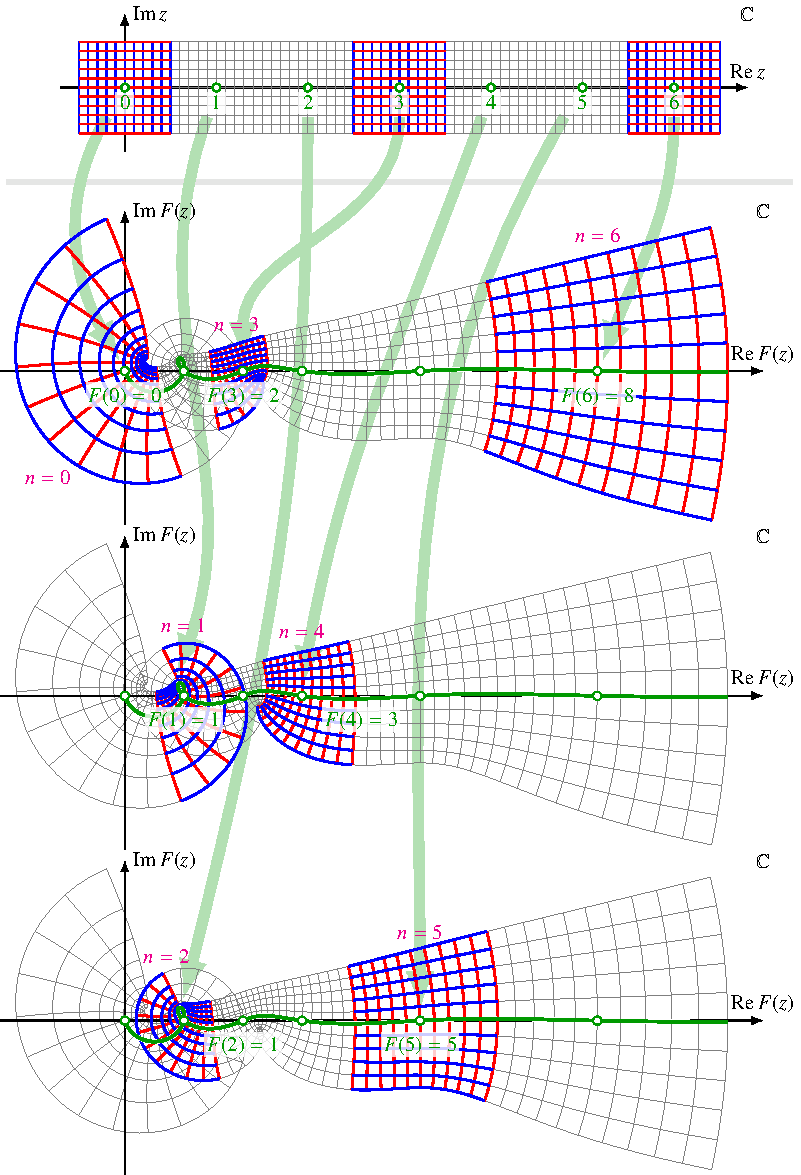
\includegraphics[width=0.82\textwidth]{chapters/040-rekursion/images/fibonacci.pdf}
\caption{Komplexe Fibonacci-Zahlen-Funktion $F(z)$ von
\eqref{buch:rekursion:linear:fibonaccifunktion}
dargestellt als Abbildung $\mathbb{C}\to\mathbb{C}$.
Die ganzzahligen $z$ werden auf die wohlbekannten Fibonacci-Zahlen
abgebildet.
Zur besseren Lesbarkeit wird der Wertebereich dreimal dargestellt,
damit die Bilder der einzelnen reellen Teilintervalle in verschiedene
Wertebereich-Bilder verteilt werden können.
$x$-Werte zwischen $3k-\frac12$ und $3k+\frac12$ werden im obersten
Bildbereich dargestellt, solche zwischen $3k+\frac12$ und $3k+\frac32$ 
im mittleren und schliesslich solche zwischen $3k+\frac32$ und $3k+\frac52$
im untersten.
Die reelle Achse wird auf die grüne Kurve abgebildet.
\label{buch:rekursion:linear:fibonaccigraph}}
\end{figure}
Matt Parker vom Youtube-Kanal Stand-up Maths hat in einem
\index{Matt Parker}%
\index{Parker, Matt}%
\index{Stand-up Maths}%
Video\footnote{\url{https://youtu.be/ghxQA3vvhsk}} die Lösungsfunktionen
für die Differenzengleichung der Fibonacci-Zahlen für beliebige
reelle und komplexe Argumente visualisiert.
Die Nullstellen des charakteristischen Polynoms
\[
\lambda^2-\lambda-1=0
\qquad
\Rightarrow
\qquad
\lambda_\pm = \begin{cases}
\displaystyle
\frac{1+\sqrt{5}}{2}=\varphi
\\[8pt]
\displaystyle
\frac{1-\sqrt{5}}{2}=-\frac{1}{\varphi},
\end{cases}
\]
dabei ist $\varphi$ das Verhältnis des goldenen Schnittes.
\index{goldener Schnitt}%
\index{Schnitt, goldener}%
Die Anfangsbedingungen $F(0)=0$ und $F(1)=1$ bedeutet, dass
\begin{equation}
F(z) = \frac{1}{\sqrt{5}}\varphi^z - \frac{1}{\sqrt{5}}\frac{1}{(-\varphi)^z}.
\label{buch:rekursion:linear:fibonaccifunktion}
\end{equation}
Dies ist die Funktion, die Matt Parker in seinem Video visualisiert hat.
Abbildung~\eqref{buch:rekursion:linear:fibonaccigraph} zeigt die Abbildung
$z\mapsto F(z)$.
Allerdings sind die Funktionen
\[
F_{kl}(z)
=
\frac{1}{\sqrt{5}}
\varphi^ze^{2k\pi iz}
-
\frac{1}{\sqrt{5}(-\varphi)^z} e^{2l\pi iz}
\]
ebenfalls Lösungen der Differenzengleichung mit den gleichen 
Anfangswerten.




%
% 4-hypergeometrisch.tex
%
% (c) 2021 Prof Dr Andreas Müller, OST Ostschweizer Fachhochschule
%
\section{Hypergeometrische Funktionen
\label{buch:rekursion:section:hypergeometrische-funktion}}
%\kopfrechts{Hypergeometrische Funktionen}
Kann man eine Formel für die Lösung $S_n$ der lineare Differenzengleichung
\[
n^3S_{n}
=
16(n-{\textstyle\frac12})(2n^2-2n+1)S_{n-1}
-256(n-1)^3S_3
\]
mit Anfangswerten $S_0=1$ und $S_1=8$ angeben?
Dies scheint auf den ersten Blick unmöglich kompliziert, man kann aber
zeigen, dass
\begin{equation}
S_n
=
\sum_{k=0}^n 
\binom{2n-2k}{n-k}^2 \binom{2k}{k}^2
\label{buch:rekursion:hypergeometrisch:eqn:Sn}
\end{equation}
gilt (\cite[p.~xi]{buch:ab}).
Die Lösung ist also eine Summe von Summanden, die sehr viel einfacher
aussehen und vor allem die besondere Eigenschaft haben, dass die
Quotienten aufeinanderfolgender Terme rationale Funktionen von $k$
sind.

\kopfrechts{Hypergeometrische Funktionen}

\begin{definition}
Ein Folge heisst {\em hypergeometrisch}, wenn der Quotient aufeinanderfolgender
\index{hypergeometrische Folge}%
\index{Folge, hypergeometrisch}%
Terme eine rationale Funktion des Folgenindex ist.
\end{definition}

Die Koeffizienten der Potenzreihenentwicklungen aller bisher behandelten
speziellen Funktionen waren hypergeometrisch.
Im aktuellen Abschnitt soll daher die Klasse der sogenannten
hypergeometrischen Funktionen untersucht werden, die durch diese
Eigenschaft charakterisiert sind.

In Abschnitt~\ref{buch:rekursion:hypergeometrisch:binomialkoeffizienten}
wird klar werden, dass Folgen, deren Terme aus Fakultäten und
Binomialkoeffizienten immer hypergeometrisch sind.
\index{Binomialkoeffizient}%
Die Untersuchung der geometrischen Reihe in
Abschnitt~\ref{buch:rekursion:hypergeometrisch:geometrisch}
\index{geometrische Reihe}%
\index{Reihe, geometrische}%
motiviert die Namensgebung.
Abschnitt~\ref{buch:rekursion:hypergeometrisch:reihen}
definiert den Begriff der hypergeometrischen Reihe und zeigt, 
wie sie in eine Standardform gebracht werden können.
In Abschnitt~\ref{buch:rekursion:hypergeometrisch:beispiele}
schliesslich wird an Hand von Beispielen gezeigt, wie bekannte
Funktionen als hypergeometrische Funktionen interpretiert werden können.

%
% Quotienten von Binomialkoeffizienten
%
\subsection{Quotienten von Binomialkoeffizienten
\label{buch:rekursion:hypergeometrisch:binomialkoeffizienten}}
Aufeinanderfolgende Terme der Summe
\eqref{buch:rekursion:hypergeometrisch:eqn:Sn}
sollen als Quotienten eine rationale Funktion haben.
Dies ist eine allgemeine Eigenschaft von Folgen, die durch Fakultäten
oder Binomialkoeffizienten definiert sind, wie die beiden folgenden
Sätze zeigen.

\begin{satz}
\index{Satz!Quotienten von Fakultäten}%
\label{buch:rekursion:hypergeometrisch:satz:fakquo}
Der Quotient aufeinanderfolgender Folgenglieder
der Folge $c_k=(a+bk)!$ ist der ein Polynom vom Grad $b$.
\end{satz}
\begin{proof}[Beweis]
\begin{align*}
\frac{c_{k+1}}{c_k}
&=
\frac{(a+b(k+1))!}{(a+bk)!}
=
\frac{(a+bk+b)!}{(a+b)!}
\\
&=
(a+bk+1)(a+bk+2)\cdots(a+bk+b)
=
(a+bk+1)_b.
\end{align*}
Das Pochhammer-Symbol hat $b$ Faktoren, es ist ein Polynom vom Grad $b$.
\end{proof}
\index{Pochhammer-Symbol}%

\begin{satz}
\index{Satz!Quotienten von Binomialkoeffizienten}%
\label{buch:rekursion:hypergeometrisch:satz:binomquo}
Die Quotienten aufeinanderfolgender Werte der Binomialkoeffizienten
\[
f_k
=
\binom{a+bk}{c+dk}
\]
ist eine rationale Funktion von $k$ mit Zähler- und Nennergrad $b$.
\end{satz}

\begin{proof}[Beweis]
Indem man die Binomialkoeffizienten mit Fakultäten als
\[
\binom{a+bk}{c+dk}
=
\frac{(a+bk)!}{(c+dk)!(a-c+(b-d)k)!}
\]
ausschreibt, findet man mit
Satz~\ref{buch:rekursion:hypergeometrisch:satz:fakquo}
für die Quotienten
\begin{align}
\frac{f_{k+1}}{f_k}
&=
\frac{(a+bk+1)_b}{(c+dk+1)_d\cdot(a-c+(b-d)k+1)_{b-d}}.
\label{buch:rekursion:eqn:binomquotient}
\end{align}
Die Pochhammer-Symbole sind Polynome vom Grad $b$, $d$ bzw.~$b-d$.
Insbesondere ist auch das Nenner-Polynom vom Grad $d+(b-d)=b$.
\end{proof}

Aus den Sätzen~\ref{buch:rekursion:hypergeometrisch:satz:fakquo}
und
\ref{buch:rekursion:hypergeometrisch:satz:binomquo}
folgt jetzt sofort, dass auch der Quotient aufeinanderfolgender
Summanden der Summe~\eqref{buch:rekursion:hypergeometrisch:eqn:Sn}
eine rationale Funktion von $k$ ist.

%
% Die geometrische Reihe
%
\subsection{Die geometrische Reihe
\label{buch:rekursion:hypergeometrisch:geometrisch}}
Die Reihe
\[
f(q)
=
\sum_{k=0}^\infty aq^k
\]
heisst die {\em geometrische Reihe} ist besonders einfache
Reihe mit einer hypergeometrischen Folge von Termen.
\index{geometrische Reihe}%
\index{Reihe!geometrische}%
Die Partialsummen 
\[
S_n
=
\sum_{k=0}^n aq^k
\]
können aus der Differenz
\begin{equation}
(1-q)S_n
=
S_n - qS_n
=
\sum_{k=0}^n aq^k
-
\sum_{k=1}^{n+1} aq^k
=
a -aq^{n+1}
\label{buch:rekursion:hypergeometrisch:eqn:qsumme}
\end{equation}
berechnet werden, die man nach
\begin{equation}
S_n 
=
a\frac{1-q^{n+1}}{1-q}
\label{buch:rekursion:hypergeometrisch:eqn:geomsumme}
\end{equation}
auflösen kann.
Für $q<1$ geht $q^n\to 0$ und damit konvergiert
$S_n$  gegen
\[
\sum_{k=0}^\infty aq^k
=
a\frac{1}{1-q}.
\]

Die geometrische Reihe ist charakterisiert dadurch, dass aufeinanderfolgende
Terme den gleichen Quotienten
\[
\frac{aq^{k+1}}{aq^k}
=
q
\]
haben.
\index{geometrische Reihe}%
\index{Reihe, geometrische}%
Die Berechnung der Summe in 
\eqref{buch:rekursion:hypergeometrisch:eqn:qsumme}
beruht darauf, dass die Multiplikation mit $q$ einen ``anderen''
Teil der Summe ergibt, der sich in der Differenz weghebt.

%
% Hypergeometrische Reihen
%
\subsection{Hypergeometrische Reihen
\label{buch:rekursion:hypergeometrisch:reihen}}
Es ist plausibel, dass eine etwas lockerere Bedingung an die
Quotienten aufeinanderfolgender Terme einer Reihe immer noch
ermöglichen wird, interessante Aussagen über die durch die
Reihe beschriebenen Funktionen zu machen.

\begin{definition}
\label{buch:rekursion:hypergeometrisch:def:allg}
Eine durch die Reihe
\[
f(x) = \sum_{k=0}^\infty a_k x^k
\]
definierte Funktion $f(x)$ heisst {\em hypergeometrisch},
wenn der Quotient aufeinanderfolgender
\index{hypergeometrisch}
\index{Reihe!hypergeometrisch}
Koeffizienten eine rationale Funktion von $k$ ist,
wenn also
\[
\frac{a_{k+1}}{a_k}
=
\frac{p(k)}{q(k)}
\]
mit Polynomen $p(k)$ und $q(k)$ ist.
\end{definition}

%
% Beispiele von hypergeometrischen Funktionen
%
\subsubsection{Beispiele von hypergeometrischen Funktionen}
Die geometrische Reihe ist natürlich eine hypergeometrische Reihe,
wobei $p(k)/q(k)=1$ ist.
Etwas interessanter ist die Exponentialfunktion, die durch die Taylor-Reihe
\index{Taylor-Reihe}%
\[
e^x = \sum_{k=0}^\infty \frac{x^k}{k!}
\]
dargestellt werden kann.
Der Quotient aufeinanderfolgender Koeffizienten ist
\[
\frac{a_{k+1}}{a_k}
=
\frac{1/(k+1)!}{1/k!}
=
\frac{k!}{(k+1)!}
=
\frac{1}{k+1},
\]
eine rationale Funktion mit Zählergrad $0$ und Nennergrad $1$.

Die Kosinus-Funktion wird durch die Taylor-Reihe
\[
\cos x = \sum_{k=0}^\infty \frac{(-1)^k}{(2k)!} x^{2k}
\]
dargestellt.
Als Potenzreihe in $x$ kann die Kosinus-Reihe nicht hypergeometrisch sein,
die ungeraden Koeffizienten verschwinden und damit undefinierte
Quotienten haben.
Als Reihe in $z=x^2$ ist aber
\[
\sum_{k=0}^\infty \frac{(-1)^k}{(2k)!} z^k
\qquad\Rightarrow\qquad
a_k = \frac{(-1)^k}{(2k)!}
\]
hypergeometrisch, weil der Quotient aufeinanderfolgender Koeffizienten
\[
\frac{a_{k+1}}{a_k}
=
\frac{(-1)^{k+1}}{(2k+2)!}\cdot \frac{(2k)!}{(-1)^k}
=
-\frac{1}{(2k+2)(2k+1)}
\]
eine rationale Funktion mit Zählergrad $0$ und Nennergrad $2$ ist.
Es gibt also eine hypergeometrische Reihe $f(z)$ derart, dass
$\cos x = f(x^2)$ ist.

%
% Die hypergeometrischen Funktione pFq
%
\subsubsection{Die hypergeometrischen Funktionen $\mathstrut_pF_q$}
Die Definition~\ref{buch:rekursion:hypergeometrisch:def:allg}
einer hypergeometrischen Funktion wie auch die Verschiedenartigkeit
der Beispiele können den Eindruck vermitteln, dass diese Klasse
von Funktionen unübersichtlich gross sein könnte.
Dem ist jedoch nicht so.
In diesem Abschnitt soll gezeigt werden, dass alle hypergeometrischen
Funktionen durch die in
Definition~\ref{buch:rekursion:hypergeometrisch:def} definierten
Funktionen $\mathstrut_pF_q$ ausgedrückt werden.
Die hypergeometrischen Funktionen können also vollständig parametrisiert
werden.

Zu diesem Zweck sei
\[
f(x)
=
\sum_{k=0}^\infty a_kx^k
\]
eine hypergeometrische Funktion und es
seien $p(k)$ und $q(k)$ zwei Polynome derart, dass
\[
\frac{a_{k+1}}{a_k} = \frac{p(k)}{q(k)}.
\]
Daraus lässt sich der Koeffizient $a_{k+1}$ als
\begin{equation}
a_{k+1}
=
\frac{p(k)}{q(k)}
\cdot
a_k
=
\frac{p(k)}{q(k)}
\cdot
\frac{p(k-1)}{q(k-1)}
\cdot
a_{k-1}
=\dots=
\frac{p(k)}{q(k)}
\frac{p(k-1)}{q(k-1)}
\cdots
\frac{p(1)}{q(1)}
\frac{p(0)}{q(0)}
a_0
\label{buch:rekursion:hypergeometrisch:ak+1}
\end{equation}
berechnen.
Alle Koeffizienten haben also den Faktor $a_0=f(0)$ gemeinsam.

Die Produkte von Quotienten $p(k)/q(k)$ sollen jetzt weiter
vereinfacht werden.
Sei $n$ der Grad von $p(k)$ und $m$ der Grad von $q(k)$.
Dazu nehmen wir an, dass $a_i$, $i=1,\dots,n$, die Nullstellen von $p(k)$ sind
und $b_j$, $j=1,\dots,m$, die Nullstellen von $q(k)$, dass man also
die Polynome als
\begin{align*}
p(k) &= s(k-a_1)(k-a_2)\cdots(k-a_n)
\\
q(k) &= (k-b_1)(k-b_2)\cdots(k-b_m)
\end{align*}
schreiben kann.
Der Faktor $s$ ist nötig, weil die Polynome $p(k)$ und $q(k)$ nicht
notwendigerweise normiert sind.

Um das Produkt der Quotienten zu vereinfachen, nehmen wir für den Moment
an, dass Zähler und Nenner vom Grad $n=m=1$ ist.
Dann ist nach 
\eqref{buch:rekursion:hypergeometrisch:ak+1}
\[
a_{k}
=
s^{k}
\frac{
(k-1-a_1) \cdots (2-a_1)(1-a_1)(0-a_1)
}{
(k-1-b_1) \cdots (2-b_1)(1-b_1)(0-b_1)
}
=
\frac{(-a_1)_k}{(-b_1)_k} s^k.
\]
Die Koeffizienten können daher als Quotienten von Pochhammer-Symbolen
geschrieben werden.
Für Polynome $p(k)$ und $q(k)$ beliebigen Grades sind die Koeffizienten
von der Form
\[
a_k
=
\frac{(-a_1)_k(-a_2)_k\cdots (-a_n)_k}{(-b_1)_k(-b_2)_k\cdots(-b_m)_k}
s^ka_0.
\]
Jede hypergeometrische Funktion kann daher in der Form
\[
f(x)
=
a_0
\sum_{k=0}^\infty
\frac{(-a_1)_k(-a_2)_k\cdots (-a_n)_k}{(-b_1)_k(-b_2)_k\cdots(-b_m)_k}
s^k
x^k
\]
geschrieben werden.

\begin{definition}
\label{buch:rekursion:hypergeometrisch:def}
Die hypergeometrische Funktion
$\mathstrut_pF_q$ ist definiert durch die Reihe
\[
\mathstrut_pF_q
\biggl(
\begin{matrix}
a_1,\dots,a_p\\
b_1,\dots,b_q
\end{matrix}
;
x
\biggr)
=
\mathstrut_pF_q(a_1,\dots,a_p;b_1,\dots,b_q;x)
=
\sum_{k=0}^\infty
\frac{(a_1)_k\cdots(a_p)_k}{(b_1)_k\cdots(b_q)_k}\frac{x^k}{k!}.
\]
\end{definition}

Da $(1)_k=k!$ hätte die Definition den Nenner $k!$ in der Reihe
auch durch eines der Pochhammer-Symbole ausdrücken können.
Wird dieser Nenner nicht gebraucht, kann man ihn durch einen 
zusätzlichen Faktor $(1)_k$ im Zähler des Bruchs von Pochhammer-Symbolen
kompensieren, wodurch sich der Grad $p$ des Zählers natürlich um $1$
erhöht.

Die oben analysierte Summe für $f(x)$ kann mit der
Definition~\ref{buch:rekursion:hypergeometrisch:def} als
\[
f(x)
=
a_0
\cdot
\mathstrut_{n+1}F_m \biggl(
\begin{matrix}
-a_1,-a_2,\dots,-a_n,1\\
-b_1,-b_2,\dots,-a_m
\end{matrix}; sx
\biggr)
\]
beschrieben werden.

%
% Elementare Rechenregeln
%
\subsubsection{Elementare Rechenregeln}
Die Funktionen $\mathstrut_pF_q$ sind nicht alle unabhängig.
In Abschnitt~\ref{buch:rekursion:hypergeometrisch:stammableitung}
wird gezeigt werden, dass Ableitung und Stammfunktion einer hypergeometrischen
Funktion durch Manipulation der Parameter $a_k$ und $b_k$ bestimmt werden
können.
Viel einfacher sind jedoch die folgenden, aus
Definition~\ref{buch:rekursion:hypergeometrisch:def}
offensichtlichen Regeln:

\begin{satz}[Permutationsregel]
\index{Permutationsregel}%
\index{Satz!Permutationsregel für hypergeometrische Funktionen}%
\label{buch:rekursion:hypergeometrisch:satz:permuationsregel}
Sei $\pi$ eine beliebige Permutation der Zahlen $1,\dots,p$ und $\sigma$ eine
beliebige Permutation der Zahlen $1,\dots,q$, dann ist 
\begin{equation}
\mathstrut_pF_q\biggl(
\begin{matrix}
a_1,\dots,a_p\\b_1,\dots,a_q
\end{matrix}
;x
\biggr)
=
\mathstrut_pF_q\biggl(
\begin{matrix}
a_{\pi(1)},\dots,a_{\pi(p)}\\b_{\sigma(1)},\dots,b_{\sigma(q)}
\end{matrix}
;x
\biggr).
\label{buch:rekursion:hypergeometrisch:eqn:permuationsregel}
\end{equation}
\end{satz}

\begin{satz}[Kürzungsformel]
\index{Kürzungsregel}%
\index{Satz!Kürzungsformel für hypergeometrische Funktionen}%
\label{buch:rekursion:hypergeometrisch:satz:kuerzungsregel}
Stimmt einer der Koeffizienten $a_k$ mit einem der Koeffizienten $b_i$
überein, dann können beide weggelassen werden:
\begin{equation}
\mathstrut_{p+1}F_{q+1}\biggl(
\begin{matrix}
c,a_1,\dots,a_p\\
c,b_1,\dots,b_q
\end{matrix};
x
\biggr)
=
\mathstrut_{p}F_{q}\biggl(
\begin{matrix}
a_1,\dots,a_p\\
b_1,\dots,b_q
\end{matrix};
x
\biggr).
\label{buch:rekursion:hypergeometrisch:eqn:kuerzungsregel}
\end{equation}
\end{satz}

%
% Beispiele von hypergeometrischen Funktionen
%
\subsection{Beispiele von hypergeometrischen Funktionen
\label{buch:rekursion:hypergeometrisch:beispiele}}
Viele der bekannten Reihenentwicklungen häufig verwendeter Funktionen
lassen sich durch die hypergeometrischen Funktionen von
Definition~\ref{buch:rekursion:hypergeometrisch:def} ausdrücken.
In diesem Abschnitt werden einige Beispiel dazu gegeben.

%
% Die geometrische Reihe
%
\subsubsection{Die geometrische Reihe}
In der geometrischen Reihe fehlt der Nenner $k!$, es braucht
daher einen Term $(1)_k$ im Zähler, um den Nenner zu kompensieren.
Somit ist die geometrische Reihe
\[
\frac{a}{1-x}
=
\sum_{k=0}^\infty
ax^k
=
a\sum_{k=0}^\infty
\frac{(1)_k}{1}
\frac{x^k}{k!}
=
a\cdot\mathstrut_1F_0\biggl(\begin{matrix}1\\\text{---}\end{matrix};x\biggr).
\]

%
% Die Exponentialfunktion
%
\subsubsection{Exponentialfunktion}
\index{Exponentialfunktion}%
Die Exponentialfunktion ist die Reihe
\[
e^x = \sum_{k=0}^\infty \frac{x^k}{k!}.
\]
In diesem Fall werden keine Quotienten von Pochhammer-Symbolen
benötigt, es ist daher
\[
e^x = \mathstrut_0F_0(x).
\]

%
% Wurzelfunktionen
%
\subsubsection{Wurzelfunktionen}
\index{Wurzelfunktion}%
Die Wurzelfunktion $x\mapsto \sqrt{x}$ hat keine Taylor-Entwicklung
in $x=0$, aber die Funktion $x\mapsto\sqrt{1+x}$ hat die Taylor-Reihe
\[
\sqrt{1+x}
=
1
+
\frac12 x
-
\frac{1\cdot 1}{2\cdot 4}x^2
+
\frac{1\cdot 1\cdot 3}{2\cdot 4\cdot 6}x^3
-
\frac{1\cdot 1\cdot 3\cdot 5}{2\cdot 4\cdot 6\cdot 8}x^4
+
\dots
\]
Um die Verbindung zu einer hypergeometrischen Funktion herzustellen,
müssen wir den Term $x^k/k!$ abspalten.
Dann wird
\begin{align*}
\sqrt{1+x}
&=
1
+
\frac12 \frac{x}{1!}
-
\frac{1\cdot 1}{2^2}\frac{x^2}{2!}
+
\frac{1\cdot 1\cdot 3}{2^3}\frac{x^3}{3!}
-
\frac{1\cdot 1\cdot 3\cdot 5}{2^4}\frac{x^4}{4!}
+
\dots
\\
&=
1
+
\frac12 \cdot\frac{x}{1!}
-
\frac{1}{2}\cdot \frac{1}{2}\cdot\frac{x^2}{2!}
+
\frac{1}{2}\cdot \frac{1}2\cdot \frac{3}{2}\cdot\frac{x^3}{3!}
-
\frac{1}{2}\cdot \frac{1}{2}\cdot \frac{3}{2}\cdot \frac{5}{2}\cdot\frac{x^4}{4!}
+
\dots
\end{align*}
Es ist noch etwas undurchsichtig, warum die ersten beiden Terme
das gleiche Vorzeichen haben und warum der Faktor $\frac12$ in jedem
Term zweimal vorkommt.
Diese Unklarheit kann jedoch beseitigt werden, wenn man den ersten
Faktor als $-\frac12$ schreibt:
\begin{align*}
\sqrt{1+x}
&=
1
-
\biggl(-\frac12\biggr)\cdot\frac{x}{1!}
+
\biggl(-\frac{1}{2}\biggr)\cdot \frac{1}{2}\cdot\frac{x^2}{2!}
-
\biggl(-\frac{1}{2}\biggr)\cdot \frac{1}2\cdot \frac{3}{2}\cdot\frac{x^3}{3!}
+
\biggl(-\frac{1}{2}\biggr)\cdot \frac{1}{2}\cdot \frac{3}{2}\cdot \frac{5}{2}\cdot\frac{x^4}{4!}
+
\dots
\\
&=
1 + 
\biggl(-\frac12\biggr)\cdot\frac{-x}{1!}
+
\biggl(-\frac{1}{2}\biggr)\cdot \frac{1}{2}\cdot\frac{(-x)^2}{2!}
+
\biggl(-\frac{1}{2}\biggr)\cdot \frac{1}2\cdot \frac{3}{2}\cdot\frac{(-x)^3}{3!}
+
\biggl(-\frac{1}{2}\biggr)\cdot \frac{1}{2}\cdot \frac{3}{2}\cdot \frac{5}{2}\cdot\frac{(-x)^4}{4!}
+
\dots
\end{align*}
Die Koeffizienten sind aufsteigende Produkte mit $k$ Faktoren, die alle bei
$-\frac12$ beginnen, sie können daher als Pochhammer-Symbole $(-\frac12)_k$
geschrieben werden.
Die Wurzelfunktion ist daher die hypergeometrische Funktion
\[
\sqrt{1\pm x}
=
\sum_{k=0}^\infty
\biggl(-\frac12\biggr)_k \frac{(\pm x)^k}{k!}
=
\mathstrut_1F_0\biggl(
\begin{matrix}-\frac12\\\text{---}\end{matrix};\mp x
\biggr).
\]
Mit der Newtonschen Binomialreihe, die in 
\index{Binomialreihe}%
\index{Newtonsche Reihe}%
Abschnitt~\ref{buch:differentialgleichungen:subsection:newtonschereihe}
hergleitet wird,
kann man ganz analog jede beliebige Wurzelfunktion
\begin{align*}
(1+x)^\alpha
&=
1+\alpha x + \frac{\alpha(\alpha-1)}{2!}x^2 + \frac{\alpha(\alpha-1)(\alpha-2)}{3!}x^3+\dots
%\\
%&
=
\sum_{k=0}^\infty \frac{(-\alpha)_k}{k!}x^k
=
\mathstrut_1F_0\biggl(\begin{matrix}-\alpha\\\text{---}\end{matrix};-x\biggr)
\end{align*}
durch $\mathstrut_1F_0$ ausdrücken.
Dieses Resultat ist der Inhalt von
Satz~\ref{buch:differentialgleichungen:satz:newtonschereihe}.


%
% Logarithmusfunktion
%
\subsubsection{Logarithmusfunktion}
\index{Logarithmusfunktion}%
Für $x\in (-1,1)$ konvergiert die Taylor-Reihe
\[
\log(1+x)
=
x-\frac{x^2}{2}+\frac{x^3}{3}-\frac{x^4}{4}+\dots
\]
der Logarithmusfunktion im Punkt $x=0$.
Die Reihe beginnt nicht mit einem konstanten Term, daher klammern wir
zunächst einen Faktor $x$ aus:
\[
\log(1+x)
=
x\cdot
\biggl(
1-\frac{x}{2}+\frac{x^2}{3}-\frac{x^3}{4}+\dots
\biggr).
\]
Um dies in die Form einer hypergeometrischen Funktion zu bringen,
muss zunächst wieder der Nenner $k!$ hergestellt werden:
\begin{align*}
\log(1+x)
&=
x\cdot\biggl(
1
- \frac{1!}{2} \frac{x}{1!}
+ \frac{2!}{3} \frac{x^2}{2!} 
- \frac{3!}{4} \frac{x^3}{3!}+\dots
\biggr).
\intertext{Den Nenner $k+1$ kann man als Quotienten $k!/(k+1)!$ erhalten,
also}
\log(1+x)
&=
x\cdot\biggl(
1
- \frac{(1!)^2}{2!} \frac{x}{1!}
+ \frac{(2!)^2}{3!} \frac{x^2}{2!} 
- \frac{(3!)^2}{4!} \frac{x^3}{3!}+\dots
\biggr).
\end{align*}
Die Fakultät
\[
(k+1)!
=
1\cdot 2 \cdot 3 \cdot\ldots\cdot k\cdot (k+1)
=
2 \cdot (2 + 1) \cdot (2+2) \cdot\ldots\cdot (2+k-2) \cdot (2+k-1)
=
(2)_{k}
\]
ist auch ein Pochhammer-Symbol, so dass die Logarithmusfunktion
zur hypergeometrischen Funktion
\[
\log(1+x)
=
x\cdot\biggl(
1
+ \frac{(1)_1(1)_1}{(2)_1} \frac{(-x)}{1!}
+ \frac{(1)_2(1)_2}{(2)_2} \frac{(-x)^2}{2!} 
+ \frac{(1)_3(1)_3}{(2)_2} \frac{(-x)^3}{3!}+\dots
\biggr)
=
x\cdot
\mathstrut_2F_1\biggl(\begin{matrix}1,1\\2\end{matrix};-x\biggr)
\]
wird.

%
% Trigonometrische Funktionen
%
\subsubsection{Trigonometrische Funktionen}
\index{trigonometrische Funktionen!als hypergeometrische Funktionen}%
Die Kosinus-Funktion wurde bereits als hypergeometrische Funktion erkannt,
im Folgenden soll dies auch noch für die Sinus-Funktion
durchgeführt werden.
Die Taylor-Reihe der Sinus-Funktion im Punkt $0$ ist
\begin{align*}
\sin x
&=
x-\frac{x^3}{3!}+\frac{x^5}{5!}-\frac{x^7}{7!}+\dots
\end{align*}
In dieser Reihe fehlen die geraden Potenzen, wir Klammern daher einen
Faktor $x$ aus und schreiben den Rest als eine Funktion von $-x^2$
\begin{align*}
\sin x
&=
x
\biggl(
1+\frac{-x^2}{3!}+\frac{(-x^2)^2}{5!}-\frac{(-x^2)^3}{7!}+\dots
\biggr)
=
x f(-x^2).
\end{align*}
Die Funktion $f(z)$ soll jetzt als hypergeometrische Funktion geschrieben
werden.
Dazu muss zunächst wieder der Nenner $k!$ wiederhergestellt werden:
\begin{equation*}
f(z)
=
1
+
\frac{1!}{3!}\cdot \frac{z}{1!}
+
\frac{2!}{5!}\cdot \frac{z^2}{2!}
+
\frac{3!}{7!}\cdot \frac{z^3}{3!}
+
\dots
\end{equation*}
Die Koeffizienten $k!/(2k+1)!$ müssen jetzt durch Pochhammer-Symbole
mit jeweils $k$ Faktoren ausgedrückt werden.
Dazu muss die Fakultät $(2k+1)!$ in zwei Produkte
\[
(2k+1)!
=
2\cdot 3 \cdot 4\cdot 5\cdot \ldots \cdot 2k \cdot (2k+1)
=
\underbrace{(2\cdot 4 \cdot 6\cdot\ldots\cdot 2k)}_{\textstyle\text{gerade Faktoren}}
\cdot
\underbrace{(3\cdot 5\cdot 7\cdot \ldots \cdot (2k+1))}_{\textstyle\text{ungerade Faktoren}}
\]
aufgespaltet werden.
Diese Produkte haben zwar jeweils $k$ Faktoren, aber sie sind keine
Pochhammer-Symbole, weil die Differenz aufeinanderfolgender Faktoren 
jeweils $2$ ist.
Wir dividieren sowohl die geraden Faktoren wie auch die 
ungeraden Faktoren durch $2$, damit sich das Produkt nicht ändert,
müssen wird mit $2^{2k}$ kompensieren:
\begin{align*}
(2k+1)!
&=
2^k(1\cdot2\cdot3\cdot\ldots\cdot k)
\cdot
2^k
\biggl(
\frac{3}{2}\cdot
\frac{5}{2}\cdot
\frac{7}{2}\cdot
\ldots\cdot
\frac{2k+1}{2}
\biggr)
\\
&=
4^k
\cdot
(1)_k\cdot \biggl(\frac{3}{2}\biggr)_k.
\end{align*}
Setzt man dies in die Reihe ein, wird
\begin{equation}
f(z)
=
\sum_{k=0}^\infty
\frac{(1)_k}{(1)_k\cdot (\frac{3}{2})_k\cdot 4^k}
z^k
=
\mathstrut_1F_2\biggl(
\begin{matrix}1\\1,\frac{3}{2}\end{matrix};\frac{z}4
\biggr)
=
\mathstrut_0F_1\biggl(
\begin{matrix}\text{---}\\\frac{3}{2}\end{matrix};\frac{z}4
\biggr).
\label{buch:rekursion:hyperbolisch:eqn:hilfsfunktionf}
\end{equation}
Im letzten Schritt wurde die Kürzungsregel
\eqref{buch:rekursion:hypergeometrisch:eqn:kuerzungsregel}
von
Satz~\ref{buch:rekursion:hypergeometrisch:satz:kuerzungsregel}
angewendet.
Damit lässt sich die Sinus-Funktion als
\begin{equation}
\sin x
=
x\cdot \mathstrut_1F_2\biggl(
\begin{matrix}1\\1,\frac32\end{matrix};-\frac{x^2}4
\biggr)
=
x\cdot\mathstrut_0F_1\biggl(
\begin{matrix}\text{---}\\\frac32\end{matrix};-\frac{x^2}4
\biggr)
\label{buch:rekursion:hypergeometrisch:eqn:sinhyper}
\end{equation}
durch eine hypergeometrische Funktion ausdrücken.

%
% Hyperbolische Funktionen
%
\subsubsection{Hyperbolische Funktionen}
\index{hyperbolische Funktionen!als hypergeometrische Funktionen}%
Die für die Sinus-Funktion angewendete Methode führt auch für
die Funktion 
\begin{align*}
\sinh x
&=
\sum_{k=0}^\infty \frac{x^{2k+1}}{(2k+1)!}
%\\
%&
=
x
\,
\biggl(
1+\frac{x^2}{3!} + \frac{x^4}{5!}+\frac{x^6}{7!}+\dots
\biggr).
\intertext{Die Reihe in der Klammer lässt sich mit der Funktion
$f$ von \eqref{buch:rekursion:hyperbolisch:eqn:hilfsfunktionf}
schreiben als}
&=
x\,f(-x^2)
%=
%x\cdot\mathstrut_1F_2\biggl(
%\begin{matrix}1\\1,\frac{3}{2}\end{matrix}
%;\frac{x^2}{4}
%\biggr)
=
x\cdot\mathstrut_0F_1\biggl(
\begin{matrix}\text{---}\\\frac{3}{2}\end{matrix}
;\frac{x^2}4
\biggr).
\end{align*}
Bis auf das Vorzeichen des Arguments der hypergeometrischen Funktion
ist diese Darstellung identisch mit der von $\sin x$.
Dies illustriert die Rolle der hypergeometrischen Funktionen als
``grosse Vereinheitlichung'' der bekannten speziellen Funktionen.

%
% Tschebyscheff-Polynome
%
\subsubsection{Tschebyscheff-Polynome}
\index{Tschebyscheff-Polynome}%
Man kann zeigen, dass auch die Tschebyscheff-Polynome sich durch die
hypergeometrischen Funktionen
\begin{equation}
T_n(x)
=
\mathstrut_2F_1\biggl(
\begin{matrix}-n,n\\\frac12\end{matrix}
;
\frac12(1-x)
\biggr)
\label{buch:rekursion:hypergeometrisch:tschebyscheff2f1}
\end{equation}
ausdrücken lassen.
Beweisen kann man diese Beziehung zum Beispiel mit Hilfe der
Differentialgleichungen, denen die Funktionen genügen.
Diese Methode wird in
Abschnitt~\ref{buch:differentialgleichungen:section:hypergeometrisch}
von Kapitel~\ref{buch:chapter:differential} vorgestellt.

Die Tschebyscheff-Polynome sind nicht die einzigen Familien von Polynomen,
\index{Tschebyscheff-Polynome!als hypergeometrische Funktion}
die sich durch $\mathstrut_pF_q$ ausdrücken lassen.
Für die zahlreichen Familien von orthogonalen Polynomen, die in
Kapitel~\ref{buch:chapter:orthogonalitaet} untersucht werden,
trifft dies ebenfalls zu.
Ein Funktion
\[
\mathstrut_pF_q
\biggl(
\begin{matrix}
a_1,\dots,a_p\\
b_1,\dots,b_q
\end{matrix}
;z
\biggr)
\]
ist genau dann ein Polynom, wenn mindestens einer der Parameter
$a_k$ eine negative ganze Zahl ist.
Der Grad des Polynoms ist der kleinste Betrag der negativ ganzzahligen
Werte unter den Parametern $a_k$.

%
% Die Funktionen 0F1
%
\subsubsection{Die Funktionen $\mathstrut_0F_1$}
\begin{figure}
\centering
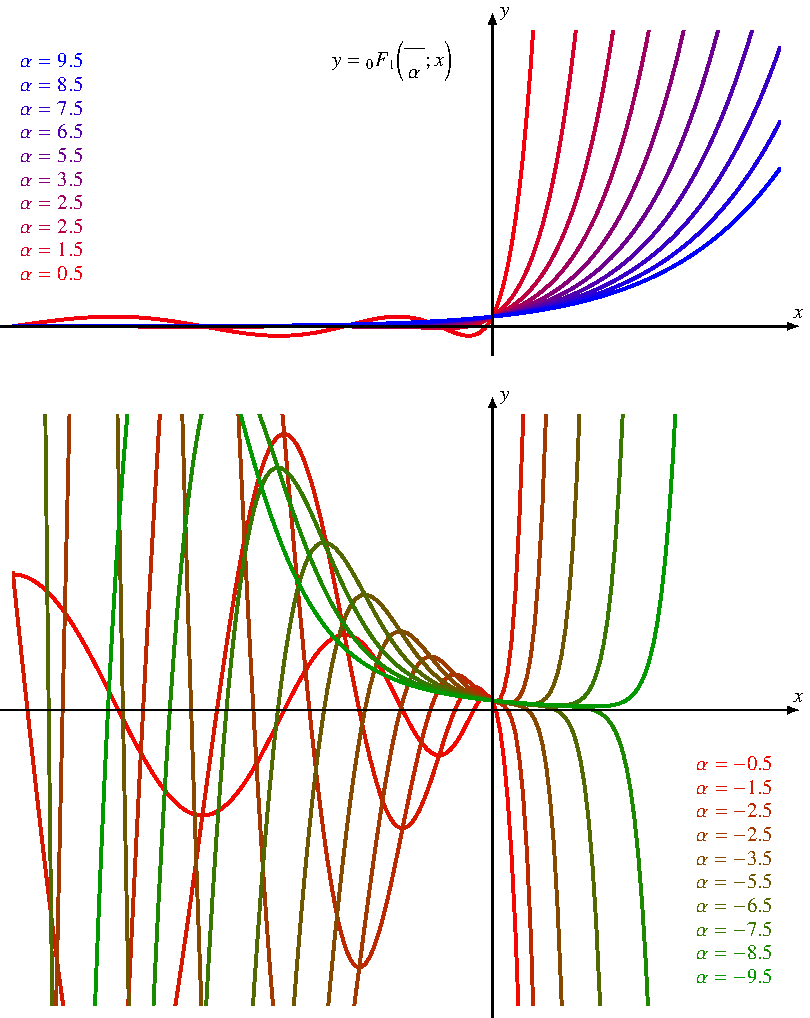
\includegraphics{chapters/040-rekursion/images/0f1.pdf}
\caption{Graphen der Funktionen $\mathstrut_0F_1(;\alpha;x)$ für
verschiedene Werte von $\alpha$.
\label{buch:rekursion:hypergeometrisch:0f1}}
\end{figure}
Die Funktionen $\mathstrut_0F_1$ sind in den Beispielen mit der
beschränkten trigonometrischen Funktion $\sin x$ und mit der
exponentiell unbeschränkten Funktion $\sinh x$ mit dem gleichen
Wert des Parameters und nur einem Wechsel des Vorzeichens des
Arguments verbunden worden.
Die Graphen der Funktionen $\mathstrut_0F_1$, die in 
Abbildung~\ref{buch:rekursion:hypergeometrisch:0f1} dargestellt sind,
machen dieses Verhalten plausibel.
Es wird sich später zeigen, dass $\mathstrut_0F_1$ auch mit den Bessel-
und den Airy-Funktionen verwandt sind.
Kapitel~\ref{chapter:0f1} zeigt Möglichkeiten der Berechnung der
Funktion $\mathstrut_0F_1$.

%
% Ableitung und Stammfunktion
%
\subsection{Ableitung und Stammfunktion hypergeometrischer Funktionen
\label{buch:rekursion:hypergeometrisch:stammableitung}}
Sowohl Ableitung wie auch Stammfunktion einer hypergeometrischen
Funktion lässt sich immer durch hypergeometrische Reihen ausdrücken.
%
% Ableitung
%
\subsubsection{Ableitung}
\index{Ableitung!hypergeometrischer Funktionen}%
Wir gehen aus von der Funktion
\begin{equation}
f(x)
=
\mathstrut_nF_m\biggl(
\begin{matrix}a_1,\dots,a_n\\b_1,\dots,b_m\end{matrix};
x\biggr)
=
\sum_{k=0}^\infty
\frac{
(a_1)_k\cdot\ldots\cdot(a_n)_k
}{
(b_1)_k\cdot\ldots\cdot(b_m)_k
}
\frac{x^k}{k!}.
\label{buch:rekursion:hypergeometrisch:eqn:f}
\end{equation}
Die Ableitung von $f(x)$ ist
\[
f'(x)
=
\sum_{k=0}^\infty
\frac{
(a_1)_k\cdot\ldots\cdot(a_n)_k
}{
(b_1)_k\cdot\ldots\cdot(b_m)_k
}
\frac{x^{k-1}}{(k-1)!}
=
\sum_{k=1}^\infty
\frac{
(a_1)_{k+1}\cdot\ldots\cdot(a_n)_{k+1}
}{
(b_1)_{k+1}\cdot\ldots\cdot(b_m)_{k+1}
}
\frac{x^k}{k!}.
\]
Der Koeffizient besteht zwar aus lauter Pochhammer-Symbolen, aber sie
haben jeweils einen Faktor zuviel.
Indem man den jeweils ersten Faktor ausklammert, kann man die
Terme wieder in die Form einer hypergeometrischen Reihe bringen.
\begin{align*}
f'(x)
&=
\sum_{k=1}^\infty
\frac{
a_1(a_1)_{k}\cdot\ldots\cdot a_n(a_n)_{k}
}{
b_1(b_1)_{k}\cdot\ldots\cdot b_m(b_m)_{k}
}
\frac{x^k}{k!}
\\
&=
\sum_{k=1}^\infty
\frac{
a_1\cdot\ldots\cdot a_n
}{
b_1\cdot\ldots\cdot b_m
}
\frac{
(a_1+1)_{k}\cdot\ldots\cdot(a_n+1)_{k}
}{
(b_1+1)_{k}\cdot\ldots\cdot(b_m+1)_{k}
}
\frac{x^k}{k!}
\\
&=
\frac{
a_1\cdot\ldots\cdot a_n
}{
b_1\cdot\ldots\cdot b_m
}
\,
\mathstrut_nF_m\biggl(
\begin{matrix}a_1+1,\dots,a_n+1\\b_1+1,\dots,b_m+1\end{matrix};
x\biggr).
\end{align*}

\begin{beispiel}
\index{Kosinus-Funktion}%
Die Kosinus-Funktion
\[
\cos x
=
1 - \frac{x^2}{2!} + \frac{x^4}{4!} - \frac{x^6}{6!} + \dots
=
\sum_{k=0}^\infty
\frac{(-1)^k}{(2k)!}x^{2k}
\]
kann wie folgt als hypergeometrische Funktion geschrieben werden.
Der Nenner hat $2k$ Faktoren, er muss also aus zwei Pochhammer-Symbolen
zusammengesetzt werden.
Dazu muss er erst um den Faktor $2^{2k}$ gekürzt werden, was
\[
\frac{(2k)!}{2^{2k}}
=
\frac12\cdot\frac32\cdot\frac52\cdot\ldots\cdot\frac{2k-1}2
\cdot
\frac22\cdot\frac42\cdot\frac62\cdot\ldots\cdot\frac{2k}2
=
({\textstyle\frac12})_k\cdot k!.
\]
Damit kann jetzt die Kosinus-Funktion als
\begin{align*}
\cos x
&=
\sum_{k=0}^\infty
\frac{2^k}{(2k)!}\biggl(\frac{-x^2}{4}\biggr)^k
=
\sum_{k=0}^\infty
\frac{1}{(\frac12)_k}
\frac{1}{k!}\biggl(\frac{-x^2}{4}\biggr)^k
=
\mathstrut_0F_1\biggl(\begin{matrix}\text{---}\\\frac12\end{matrix};-\frac{x^2}4\biggr)
\end{align*}
geschrieben werden kann.

Die Ableitung der Kosinus-Funktion ist daher
\begin{align*}
\frac{d}{dx} \cos x
&=
\frac{d}{dx}
\mathstrut_0F_1\biggl(
\begin{matrix}\text{---}\\\frac12\end{matrix};-\frac{x^2}4
\biggr)
=
\frac{1}{\frac12}
\,
\mathstrut_0F_1\biggl(
\begin{matrix}\text{---}\\\frac32\end{matrix};-\frac{x^2}4
\biggr)
\cdot\biggl(-\frac{x}2\biggr)
=
-x
\cdot
\mathstrut_0F_1\biggl(
\begin{matrix}\text{---}\\\frac32\end{matrix};-\frac{x^2}4
\biggr).
\intertext{Dies stimmt mit der in
\eqref{buch:rekursion:hypergeometrisch:eqn:sinhyper}
gefundenen Darstellung der Sinusfunktion mit Hilfe der hypergeometrischen
Funktion $\mathstrut_0F_1$ überein, es ist also wie erwartet}
&=-\sin x.
\qedhere
\end{align*}
\end{beispiel}

%
% Stammfunktion
%
\subsubsection{Stammfunktion}
\index{Stammfunktion!hypergeometrischer Funktionen}%
Eine Stammfunktion kann man auf die gleiche Art und Weise wie
die Ableitung finden.
Termweises Integrieren der Funktion
\eqref{buch:rekursion:hypergeometrisch:eqn:f}
ergibt
\begin{align}
\int f(x)\,dx
&=
\sum_{k=0}^\infty
\frac{
(a_1)_k\cdot\ldots\cdot(a_n)_k
}{
(b_1)_k\cdot\ldots\cdot(b_m)_k
}
\frac{x^{k+1}}{(k+1)!}.
\notag
\intertext{Wieder muss man die Pochhammer-Symbole durch solche mit
einem zusätzlichen Faktor schreiben.
Dies ist möglich, wenn keiner der Parameter $a_i=1$ und $b_j=1$
ist.
Die Stammfunktion wird daher
}
&=
\sum_{k=1}^\infty
\frac{
(a_1-1)(a_1)_k
\cdot\ldots\cdot
(a_n-1)(a_n)_k
}{
(b_1-1)(b_1)_k
\cdot\ldots\cdot
(b_m-1)(b_m)_k
}
\frac{x^k}{k!}
\notag
\\
&=
\sum_{k=1}^\infty
\frac{
(a_1-1)_{k+1}
\cdot\ldots\cdot
(a_n-1)_{k+1}
}{
(b_1-1)_{k+1}
\cdot\ldots\cdot
(b_m-1)_{k+1}
}
\frac{x^k}{k!}
\label{buch:rekursion:hypergeometrisch:eqn:stammfunktion:summe}
\\
&=
\mathstrut_nF_m\biggl(
\begin{matrix}
a_1-1,\dots,a_n-1\\
b_1-1,\dots,b_m-1
\end{matrix}
;x
\biggr)
-
\frac{(a_1-1)\dots(a_n-1)}{(b_1-1)\dots(b_m-1)}.
\notag
\end{align}
Der Term auf der rechten Seite kompensiert den konstanten
Term, der in der hypergeometrischen Funktion $\mathstrut_nF_m$
vorkommt, aber nicht in der
Summe~\eqref{buch:rekursion:hypergeometrisch:eqn:stammfunktion:summe}.

%
% Berechnung hypergeometrischer Funktionen
%
\subsection{Numerische Berechnung}
\begin{figure}
\centering
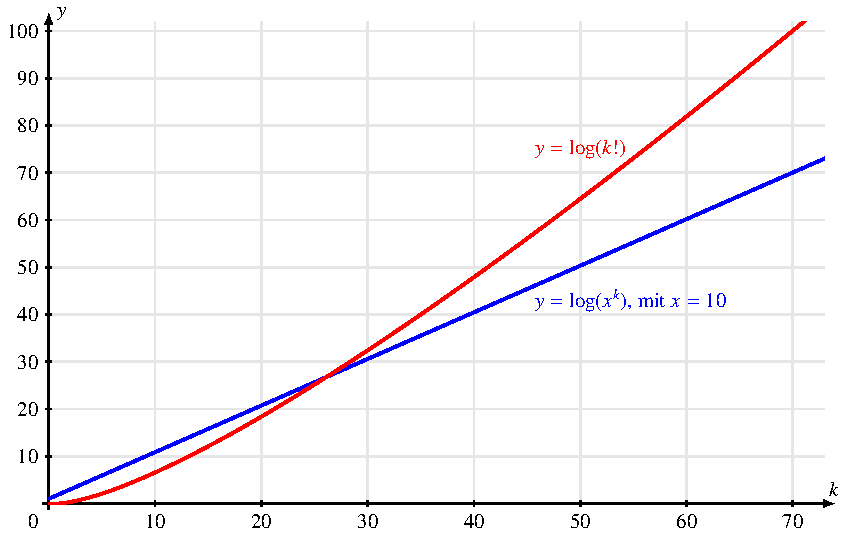
\includegraphics{chapters/040-rekursion/images/powergamma.pdf}
\caption{Anwachsen von Zähler $x^k$ und Nenner $k!$ in der
Exponentialreihe für $x=10$. 
Ab $k\approx 30$ werden die Terme der Reihe zunehmend kleiner,
was schliesslich zu Konvergenz der Reihe führt.
Für $k\approx 50$ sind die einzelnen Terme kleiner als die
Maschinengenauigkeit darzustellen gestattet.
Für negative $x$ wird starke Auslöschung die Genauigkeit des Resultates
unbrauchbar machen.
\label{buch:rekursion:hypergeometrisch:fig:powergamma}}
\end{figure}
Die naheliegendste Methode zur Berechnung einer hypergeometrischen
Funktion  $\mathstrut_pF_q$ ist die Auswertung der Potenzreihe.
Schon die einfachste hypergeometrische Funktion $\mathstrut_0F_0(x)=e^x$
zeigt aber, dass dabei numerische Schwierigkeiten auftreten können.
Für negative Argumente wird die Summe der Potenzreihe sehr klein.
Dies ist möglich, weil der Nenner $k!$ in der Potenzreihe
\[
\mathstrut_0F_0(x)
=
e^x
= 
1+x+\frac{x^2}{2!} + \frac{x^3}{3!} + \dots + \frac{x^k}{k!}+\dots
\]
sehr viel schneller anwächst als der Zähler $x^k$
(Abbildung~\ref{buch:rekursion:hypergeometrisch:fig:powergamma}).
Dazu muss aber $k$ eine gewisse Grösse haben, für $x=10$ muss
z.~B.~$k\gtrapprox30$ sein.
Für negative $x$ ist $e^x$ sehr klein, aber einzelne Terme in der
Summe sind viele Grössenordnungen grösser, was zu Auslöschung führt.

Im Falle der Exponentialfunktion gibt es eine einfache Lösung für
dieses Problem.
Um $y=e^x$ für negatives $x$ zu berechnen, verwendet man mit Vorteil
$y=1/e^{-x}$. Da $-x$ positiv ist, entsteht keine Auslöschung und der
Kehrwert führt ebenfalls keine weiteren Fehler ein.
So ist die Berechnung von $e^x$ auch für negative $x$ mit hoher
Genauigkeit möglich.

Ein ähnliches Phänomen muss ganz offensichtlich auch bei den
trigonometrischen Funktion $\sin x$ und $\cos x$ für beliebige
reelle Argumente auftreten.
Da diese Funktionen beschränkt sind, muss für grosse Absolutwerte
des Argumentes Auslöschung auftreten.
\index{Auslöschung}%
In diesem Fall können die Periodizität und goniometrische
\index{Periodizität}%
Identitäten verwendet werden, um die Berechnungsaufgabe in eine zu
transformieren, die mit hoher Genauigkeit ausgeführt werden kann.

Die allgemeine Theorie der hypergeometrischen Funktionen stellt
eine Reihe ähnlicher Transformationen bereit, die bei der Berechnung
ebenfalls hilfreich sein können.
Die Darstellung dieser Transformationen würde den Rahmen dieses
Buches sprengen.
Eine speziell interessante Technik, der Gausssche Kettenbruch,
\index{Gaussscher Kettenbruch}%
\index{Kettenbruch!Gaussscher}%
erlaubt Darstellungen einer Funktion als Kettenbruch zu finden, die
oft sehr gute numerische Eigenschaften haben.
Kapitel~\ref{chapter:0f1} untersucht einige dieser Möglichkeiten.


%\subsection{TODO}
%\begin{itemize}
%\item Hypergeometrische Transformationen
%\item Gausscher Kettenbruch \url{https://en.wikipedia.org/wiki/Gauss\%27s_continued_fraction}
%\end{itemize}


\section*{Übungsaufgaben}
\rhead{Übungsaufgaben}
\aufgabetoplevel{chapters/040-rekursion/uebungsaufgaben}
\begin{uebungsaufgaben}
%\uebungsaufgabe{0}
\uebungsaufgabe{404}
\uebungsaufgabe{402}
\uebungsaufgabe{403}
\uebungsaufgabe{401}
\uebungsaufgabe{405}
\end{uebungsaufgaben}

